\documentclass{experimentreport}

\usepackage{listings}
\usepackage{xcolor}

\definecolor{codegreen}{rgb}{0,0.6,0}
\definecolor{codegray}{rgb}{0.5,0.5,0.5}
\definecolor{codepurple}{rgb}{0.58,0,0.82}
\definecolor{backcolour}{rgb}{0.95,0.95,0.92}
\definecolor{lightgreen}{rgb}{0,0.4,0}
\definecolor{lightred}{rgb}{0.4,0,0}

\definecolor{mygray}{gray}{.9}

% \lstdefinestyle{mystyle}{
\lstset{
    %backgroundcolor=\color{backcolour},   
    commentstyle=\color{brown},
    keywordstyle=\color{magenta},
    numberstyle=\tiny\color{codegray},
    stringstyle=\color{codepurple},
    basicstyle=\ttfamily\tiny,
    breakatwhitespace=false,         
    breaklines=true,                 
    captionpos=b,                    
    keepspaces=true,                 
    numbers=none,                    
    numbersep=5pt,                  
    showspaces=false,                
    showstringspaces=false,
    showtabs=false,                  
    tabsize=2,
    escapeinside={<@}{@>}
}

% \lstset{
% basicstyle=\ttfamily\bfseries\footnotesize,
%   morekeywords={virtualinvoke},
%   keywordstyle=,
%   ndkeywordstyle=\color{red},
%   commentstyle=\color{gray},
%   stringstyle=\color{green},
%   numbers=none,
%   breaklines=true,
%   numberstyle=\ttfamily\footnotesize\color{gray},
%   stepnumber=1,
%   numbersep=6pt,
%   backgroundcolor=\color{white},
%   tabsize=4,
%   showspaces=false,
%   showstringspaces=false,
%   xleftmargin=6pt,
%   captionpos=t
% }

\lstdefinelanguage{JavaScript}{
  keywords={typeof, new, true, false, catch, function, return, null, catch, switch, var, if, in, while, do, else, case, break, export, static, const, let, class, void, async, await, interface, extends, public, this},
  % basicstyle=\linespread{1.0}\ttfamily\footnotesize,
  % keywordstyle= \color{violet}\bfseries,
  ndkeywords={class, export, boolean, throw, implements, import, this},
  ndkeywordstyle=\color{darkgray}\bfseries,
  identifierstyle=\color{black},
  sensitive=false,
  frame=lines,
  comment=[l]{//},
  morecomment=[s]{/*}{*/},
  % commentstyle=\color{gray}\ttfamily,
  % stringstyle=\color{blue}\ttfamily,
  morestring=[b]',
  morestring=[b]"
}



\usepackage{graphicx}
\usepackage{hyperref}
\usepackage{enumitem}
\usepackage{amsmath}
\usepackage{amssymb}
\usepackage{booktabs}
\usepackage{multirow}
\usepackage{xcolor}
\usepackage{colortbl}
\usepackage{caption}
\usepackage{subcaption}

%========================
% 基本信息
%========================

\setcoursename{基础软件开发技术实践}
\setreportname{智能软件工程实验报告}

\setexperimenttitle{实验六：改进针对大模型生成代码的代码审查}

\setstudentname{\hintholder{廖正强}}
\setdepartment{\hintholder{计算学部}}
\setstudentid{\hintholder{2023112920}}

\setcourseteacher{刘佳琨}
\setinstructor{刘佳琨}

\setlablocation{\hintholder{格物213}}
\setlabtime{    \hintholder{2026/7/9}}

\begin{document}

\makereporthead

%========================
% 1. 实验目的
%========================
\section{实验目的}

实验六承接实验五，目标不是重新训练模型，而是通过\textbf{上下文增强}和\textbf{Prompt 优化}改进 DeepSeek 对 AI 生成代码 Pull Request 的代码审查能力。

实验五已经发现的核心问题：
\begin{enumerate}
    \item DeepSeek P2\_C3（Few-shot + Diff + Commit）和 P2\_C4（Few-shot + Full Early Context）在 AI PR 上严重偏向预测 \texttt{merged}，Recall 高达 0.97--0.98，但 False Positive 极多（96--98/343）。
    \item 两个 LLM 组合的 Specificity（识别 unmerged 的能力）极低，P2\_C4 仅 0.136，意味着 86.4\% 的真实未合并 PR 被误判为会合并。
    \item ROC-AUC 偏低（P2\_C3: 0.581, P2\_C4: 0.632），模型对 unmerged PR 的判别能力不足。
    \item Review Comment Generation 的 BLEU/ROUGE 可计算，但低文本重合不必然代表生成质量差，需要补充风险覆盖和可操作性分析。
\end{enumerate}

因此实验六的核心改进目标是：

\begin{center}
\large\textbf{不再追求更高 Recall，而是降低模型"默认预测 merged"的过度乐观倾向，提高对 unmerged AI PR 的识别能力，并生成更有风险意识、更可操作的审查意见。}
\end{center}


%========================
% 2. 实验方法与设计
%========================
\section{实验设计}

\subsection{实验五问题回顾}

实验五在 343 条 AI 生成代码 PR 上的基线表现：

\begin{table}[htbp]
\centering
\caption{实验五基线（完整 343 条）}
\begin{tabular}{lccccc}
\toprule
组合 & Accuracy & Precision & Recall & F1 & ROC-AUC \\
\midrule
P2\_C3 & 0.7041 & 0.6933 & 0.9819 & 0.8127 & 0.5813 \\
P2\_C4 & 0.6932 & 0.6889 & 0.9731 & 0.8067 & 0.6324 \\
\bottomrule
\end{tabular}
\end{table}

\textbf{核心矛盾}：Accuracy 和 F1 看似可接受（0.69--0.81），但这完全是因为合并率 65.6\% 的数据集和模型"一律预测 merged"的策略共同制造的表象。P2\_C4 的混淆矩阵为 TN=18, FP=98, FN=6, TP=217 —— 118 个真实未合并 PR 中仅识别出 18 个。

\subsection{评估样本设计}

实验六复用实验五的 Balanced-50 AI PR 样本，包含 25 条 merged 和 25 条 unmerged PR。实验五 B01--B16 与实验六 I01--I16 均在这一固定样本上运行，因此 Prompt 与 Context 的影响可以直接比较。

\subsection{上下文增强设计}

实验六上下文增强必须遵守实验早期信息可用性约束：PR title/body、commit messages、changed files、diff/patch 可用；当前 PR 的 merge\_status、review\_decision 等审查后信息不可用。

\subsubsection{C5：Risk Checklist Context}

在 C4 基础早期上下文之上，自动生成 AI 代码风险检查清单：

\begin{itemize}
    \item 是否缺少测试文件（MISSING\_TESTS）。
    \item 是否修改文件过多（LARGE\_SCOPE，$>$10 文件）。
    \item 是否新增行数过多（LARGE\_ADDITIONS，$>$500 行）。
    \item 是否涉及配置/CI/依赖文件（CONFIG\_DEP\_CHANGE）。
    \item 是否涉及核心模块或 public API（CORE\_MODULE）。
    \item 是否 PR body 过短或模板未填写（SHORT\_DESCRIPTION）。
    \item 是否包含 AI 工具痕迹（AI\_TOOL\_TRACES：copilot、chatgpt、claude 等关键词）。
    \item 是否修改 public API 但无文档更新（API\_CHANGE\_NO\_DOCS）。
\end{itemize}

每个风险项只给出观察事实，不给出 merge 标签。这使模型在审阅前先看到潜在问题信号，对抗其"默认乐观"的倾向。

\subsubsection{C6：Repository Policy Context}

在 C5 基础上引入仓库级历史背景摘要：
\begin{itemize}
    \item 同仓库 AI PR 的历史合并率与常见未合并模式。
    \item 仓库对 AI 代码贡献的审查政策迹象。
    \item 历史评论覆盖率与审查风格摘要。
\end{itemize}

\subsubsection{C7：Historical Similar PR Context}

在 C5 基础上检索 3 条历史相似 PR 摘要：
\begin{itemize}
    \item 相同仓库优先，并综合修改规模与 title/body 关键词相似度。
    \item 展示历史 PR 的 title、变更规模与审查摘要，作为当前 PR 的对照案例。
\end{itemize}

\subsubsection{C8：Full Improved Context}

C5 + C6 + C7 + 当前 PR 信息。超长时优先保留 PR title/body、changed files summary、风险清单和核心 diff。

\subsection{Prompt 优化设计}

\subsubsection{P5：AI-Risk-Aware Prompt}

核心思想：加入 AI 生成代码专门风险清单。要求模型检查：hallucinated API、缺少测试、范围过大、描述不足、模板残留、API 变更无文档、自动化生成痕迹。输出增加 \texttt{unmerged\_risk\_score} 和 \texttt{risk\_factors} 字段。

\subsubsection{P6：Contrastive Prompt}

核心思想：强制模型分别列出支持合并的证据（merge\_evidence）和反对合并的证据（reject\_evidence），再做判断。如果两者接近，降低 merge\_probability。不允许只因为"修改小"就直接预测 merged。

\subsubsection{P7：Self-Reflection Prompt}

核心思想：模型先给初始判断，再批判性反思是否过度乐观，重新校准 merge\_probability。流程：初步预测 $\rightarrow$ 检查未合并风险 $\rightarrow$ 重新校准 $\rightarrow$ 输出最终 JSON。

\subsubsection{P8：Strict Maintainer Prompt}

核心思想：模拟严格 maintainer，对 AI 生成代码采用更高审查标准。若缺少测试、影响核心模块、PR 描述不足，应显著降低 merge\_probability。生成评论时优先指出 blocker/major 风险。

\subsection{实验矩阵}

实验六在实验五 4$\times$4 基线 (B01--B16: P1--P4 $\times$ C1--C4) 基础上，设计了完整的改进 4$\times$4 矩阵 (I01--I16: P5--P8 $\times$ C5--C8)。

\subsubsection{主实验矩阵 I01--I16}

所有16组均在同一批 50 条 AI PR 样本（复用实验五 \texttt{ai\_llm\_sample\_50.csv}）上运行，确保与 B01--B16 可比。

\begin{table}[htbp]
\centering
\caption{实验六改进矩阵 I01--I16 组合定义}
\begin{tabular}{llll}
\toprule
ID & Prompt & Context & 测试目的 \\
\midrule
I01 & P5 AI-Risk-Aware & C5 Risk Checklist & 风险清单最小增益 \\
I02 & P5 AI-Risk-Aware & C6 Repository Policy & 风险 prompt + 仓库策略 \\
I03 & P5 AI-Risk-Aware & C7 Historical PR & 风险 prompt + 历史相似 PR \\
I04 & P5 AI-Risk-Aware & C8 Full Context & 风险 prompt + 全增强上下文 \\
I05 & P6 Contrastive & C5 Risk Checklist & 正反证据 + 风险清单 \\
I06 & P6 Contrastive & C6 Repository Policy & 对比证据 + 仓库策略 \\
I07 & P6 Contrastive & C7 Historical PR & 对比证据 + 历史相似 PR \\
I08 & P6 Contrastive & C8 Full Context & 对比证据 + 全增强上下文 \\
I09 & P7 Self-Reflection & C5 Risk Checklist & 自我校准 + 风险清单 \\
I10 & P7 Self-Reflection & C6 Repository Policy & 反思 + 仓库策略 \\
I11 & P7 Self-Reflection & C7 Historical PR & 自我校准 + 历史相似 PR \\
I12 & P7 Self-Reflection & C8 Full Context & 自我校准 + 全增强上下文 \\
I13 & P8 Strict Maintainer & C5 Risk Checklist & 严格 maintainer + 风险清单 \\
I14 & P8 Strict Maintainer & C6 Repository Policy & 严格 maintainer + 仓库策略 \\
I15 & P8 Strict Maintainer & C7 Historical PR & 严格 maintainer + 历史相似 PR \\
I16 & P8 Strict Maintainer & C8 Full Context & 严格 maintainer + 完整增强上下文 \\
\bottomrule
\end{tabular}
\end{table}

调用规模：16 组 $\times$ 50 PR = 800 次 DeepSeek API 调用。

\subsection{评价指标升级}

实验六不能只看 Accuracy/F1，必须报告：
\begin{itemize}
    \item \textbf{分类指标}：Accuracy、Precision、Recall、F1、ROC-AUC、PR-AUC。
    \item \textbf{Unmerged 识别指标}：Specificity（$TN/(TN+FP)$）、Balanced Accuracy（$(Recall+Specificity)/2$）、False Positive Rate（$FP/(FP+TN)$）、Confusion Matrix。
    \item \textbf{评论质量指标}：Risk Coverage（生成评论覆盖风险清单的比例）、Actionability Rate（含可执行建议的比例）、Specificity Rate（提到具体文件/函数的比例）、Severity 分布（blocker/major 比例）。
\end{itemize}

核心成功标准：
\begin{enumerate}
    \item 相比实验五最佳基线，ROC-AUC、Specificity 或 Balanced Accuracy 提高。
    \item False Positive Rate 下降。
    \item F1 保持稳定或提高。
\end{enumerate}

%========================
% 3. 实验结果
%========================
\section{实验结果}

\subsection{主实验：I01--I16 4$\times$4 矩阵结果}

所有 I01--I16 均在实验五同一批 50 条 AI PR（25 merged + 25 unmerged）上评估，与 B01--B16 直接可比。

\begin{table}[htbp]
\centering
\caption{实验六 I01--I16 在 Balanced-50 上的完整分类指标}
\small
\begin{tabular}{lllcccccc}
\toprule
ID & Prompt & Context & Acc & F1 & AUC & Spec & BalAcc & FPR \\
\midrule
I01 & P5 & C5 & 0.6250 & 0.6897 & 0.6643 & 0.4000 & 0.6348 & 0.6000 \\
I02 & P5 & C6 & 0.6600 & 0.7018 & 0.6864 & 0.5200 & 0.6600 & 0.4800 \\
I03 & P5 & C7 & 0.6809 & 0.7273 & 0.7264 & 0.5000 & 0.6848 & 0.5000 \\
I04 & P5 & C8 & 0.6809 & 0.7368 & 0.6893 & 0.4783 & 0.6766 & 0.5217 \\
I05 & P6 & C5 & 0.6000 & 0.6875 & 0.5376 & 0.3200 & 0.6000 & 0.6800 \\
I06 & P6 & C6 & 0.6667 & 0.7333 & 0.5998 & 0.4167 & 0.6667 & 0.5833 \\
I07 & P6 & C7 & 0.6327 & 0.7097 & \textbf{0.7358} & 0.3600 & 0.6383 & 0.6400 \\
I08 & P6 & C8 & 0.6400 & 0.6897 & 0.7144 & 0.4800 & 0.6400 & 0.5200 \\
I09 & P7 & C5 & 0.5833 & 0.6774 & 0.6078 & 0.3043 & 0.5722 & 0.6957 \\
I10 & P7 & C6 & 0.6000 & 0.6667 & 0.6520 & 0.4000 & 0.6000 & 0.6000 \\
I11 & P7 & C7 & 0.6250 & 0.7000 & 0.7087 & 0.3913 & 0.6157 & 0.6087 \\
I12 & P7 & C8 & 0.6600 & 0.7213 & 0.6632 & 0.4400 & 0.6600 & 0.5600 \\
I13 & P8 & C5 & 0.6250 & 0.6667 & 0.6007 & 0.5000 & 0.6250 & 0.5000 \\
I14 & P8 & C6 & \textbf{0.7234} & \textbf{0.7547} & 0.6927 & 0.6364 & \textbf{0.7182} & 0.3636 \\
I15 & P8 & C7 & 0.5957 & 0.6275 & 0.6649 & 0.5217 & 0.5942 & 0.4783 \\
I16 & P8 & C8 & 0.6735 & 0.6800 & 0.7075 & \textbf{0.6667} & 0.6733 & \textbf{0.3333} \\
\bottomrule
\end{tabular}
\end{table}

\subsection{实验五 B01--B16 基线回顾}

作为对比，实验五已在同一批 50 条样本上完成 4$\times$4 基线：

\begin{table}[htbp]
\centering
\caption{实验五 B01--B16 基线（同一批 50 条样本）}
\small
\begin{tabular}{lllcccc}
\toprule
ID & Prompt & Context & Acc & F1 & AUC & Spec \\
\midrule
B01 & P1 & C1 & 0.4800 & 0.6486 & 0.5024 & 0.0000 \\
B02 & P1 & C2 & 0.5600 & 0.6857 & 0.5704 & 0.1600 \\
B03 & P1 & C3 & 0.5600 & 0.6765 & 0.5736 & 0.2000 \\
B04 & P1 & C4 & 0.5600 & 0.6857 & 0.6352 & 0.1600 \\
B05 & P2 & C1 & 0.5200 & 0.6757 & 0.5064 & 0.0400 \\
B06 & P2 & C2 & 0.5600 & 0.6857 & 0.5208 & 0.1600 \\
B07 & P2 & C3 & 0.5200 & 0.6571 & 0.5000 & 0.1200 \\
B08 & P2 & C4 & 0.5400 & 0.6567 & 0.5712 & 0.2000 \\
B09 & P3 & C1 & 0.4800 & 0.6061 & 0.4440 & 0.1600 \\
B10 & P3 & C2 & 0.5200 & 0.6250 & 0.5584 & 0.2400 \\
B11 & P3 & C3 & 0.5714 & 0.6557 & 0.5525 & 0.3333 \\
B12 & P3 & C4 & 0.5800 & 0.6557 & 0.5968 & 0.3600 \\
B13 & P4 & C1 & 0.4400 & 0.6111 & 0.4296 & 0.0000 \\
B14 & P4 & C2 & 0.6000 & 0.7059 & 0.5880 & 0.2400 \\
B15 & P4 & C3 & 0.5800 & 0.6957 & 0.6328 & 0.2000 \\
B16 & P4 & C4 & 0.5400 & 0.6667 & 0.5200 & 0.1600 \\
\bottomrule
\end{tabular}
\end{table}

实验五基线的核心问题清晰可见：所有 16 组 Specificity 均不高于 0.36，多数低于 0.25。B14（最佳 F1=0.7059）的 Specificity 仅 0.24，FPR 高达 0.76。模型系统性偏向预测 merged。

\begin{figure}[htbp]
\centering
\begin{subfigure}{0.48\textwidth}
    \centering
    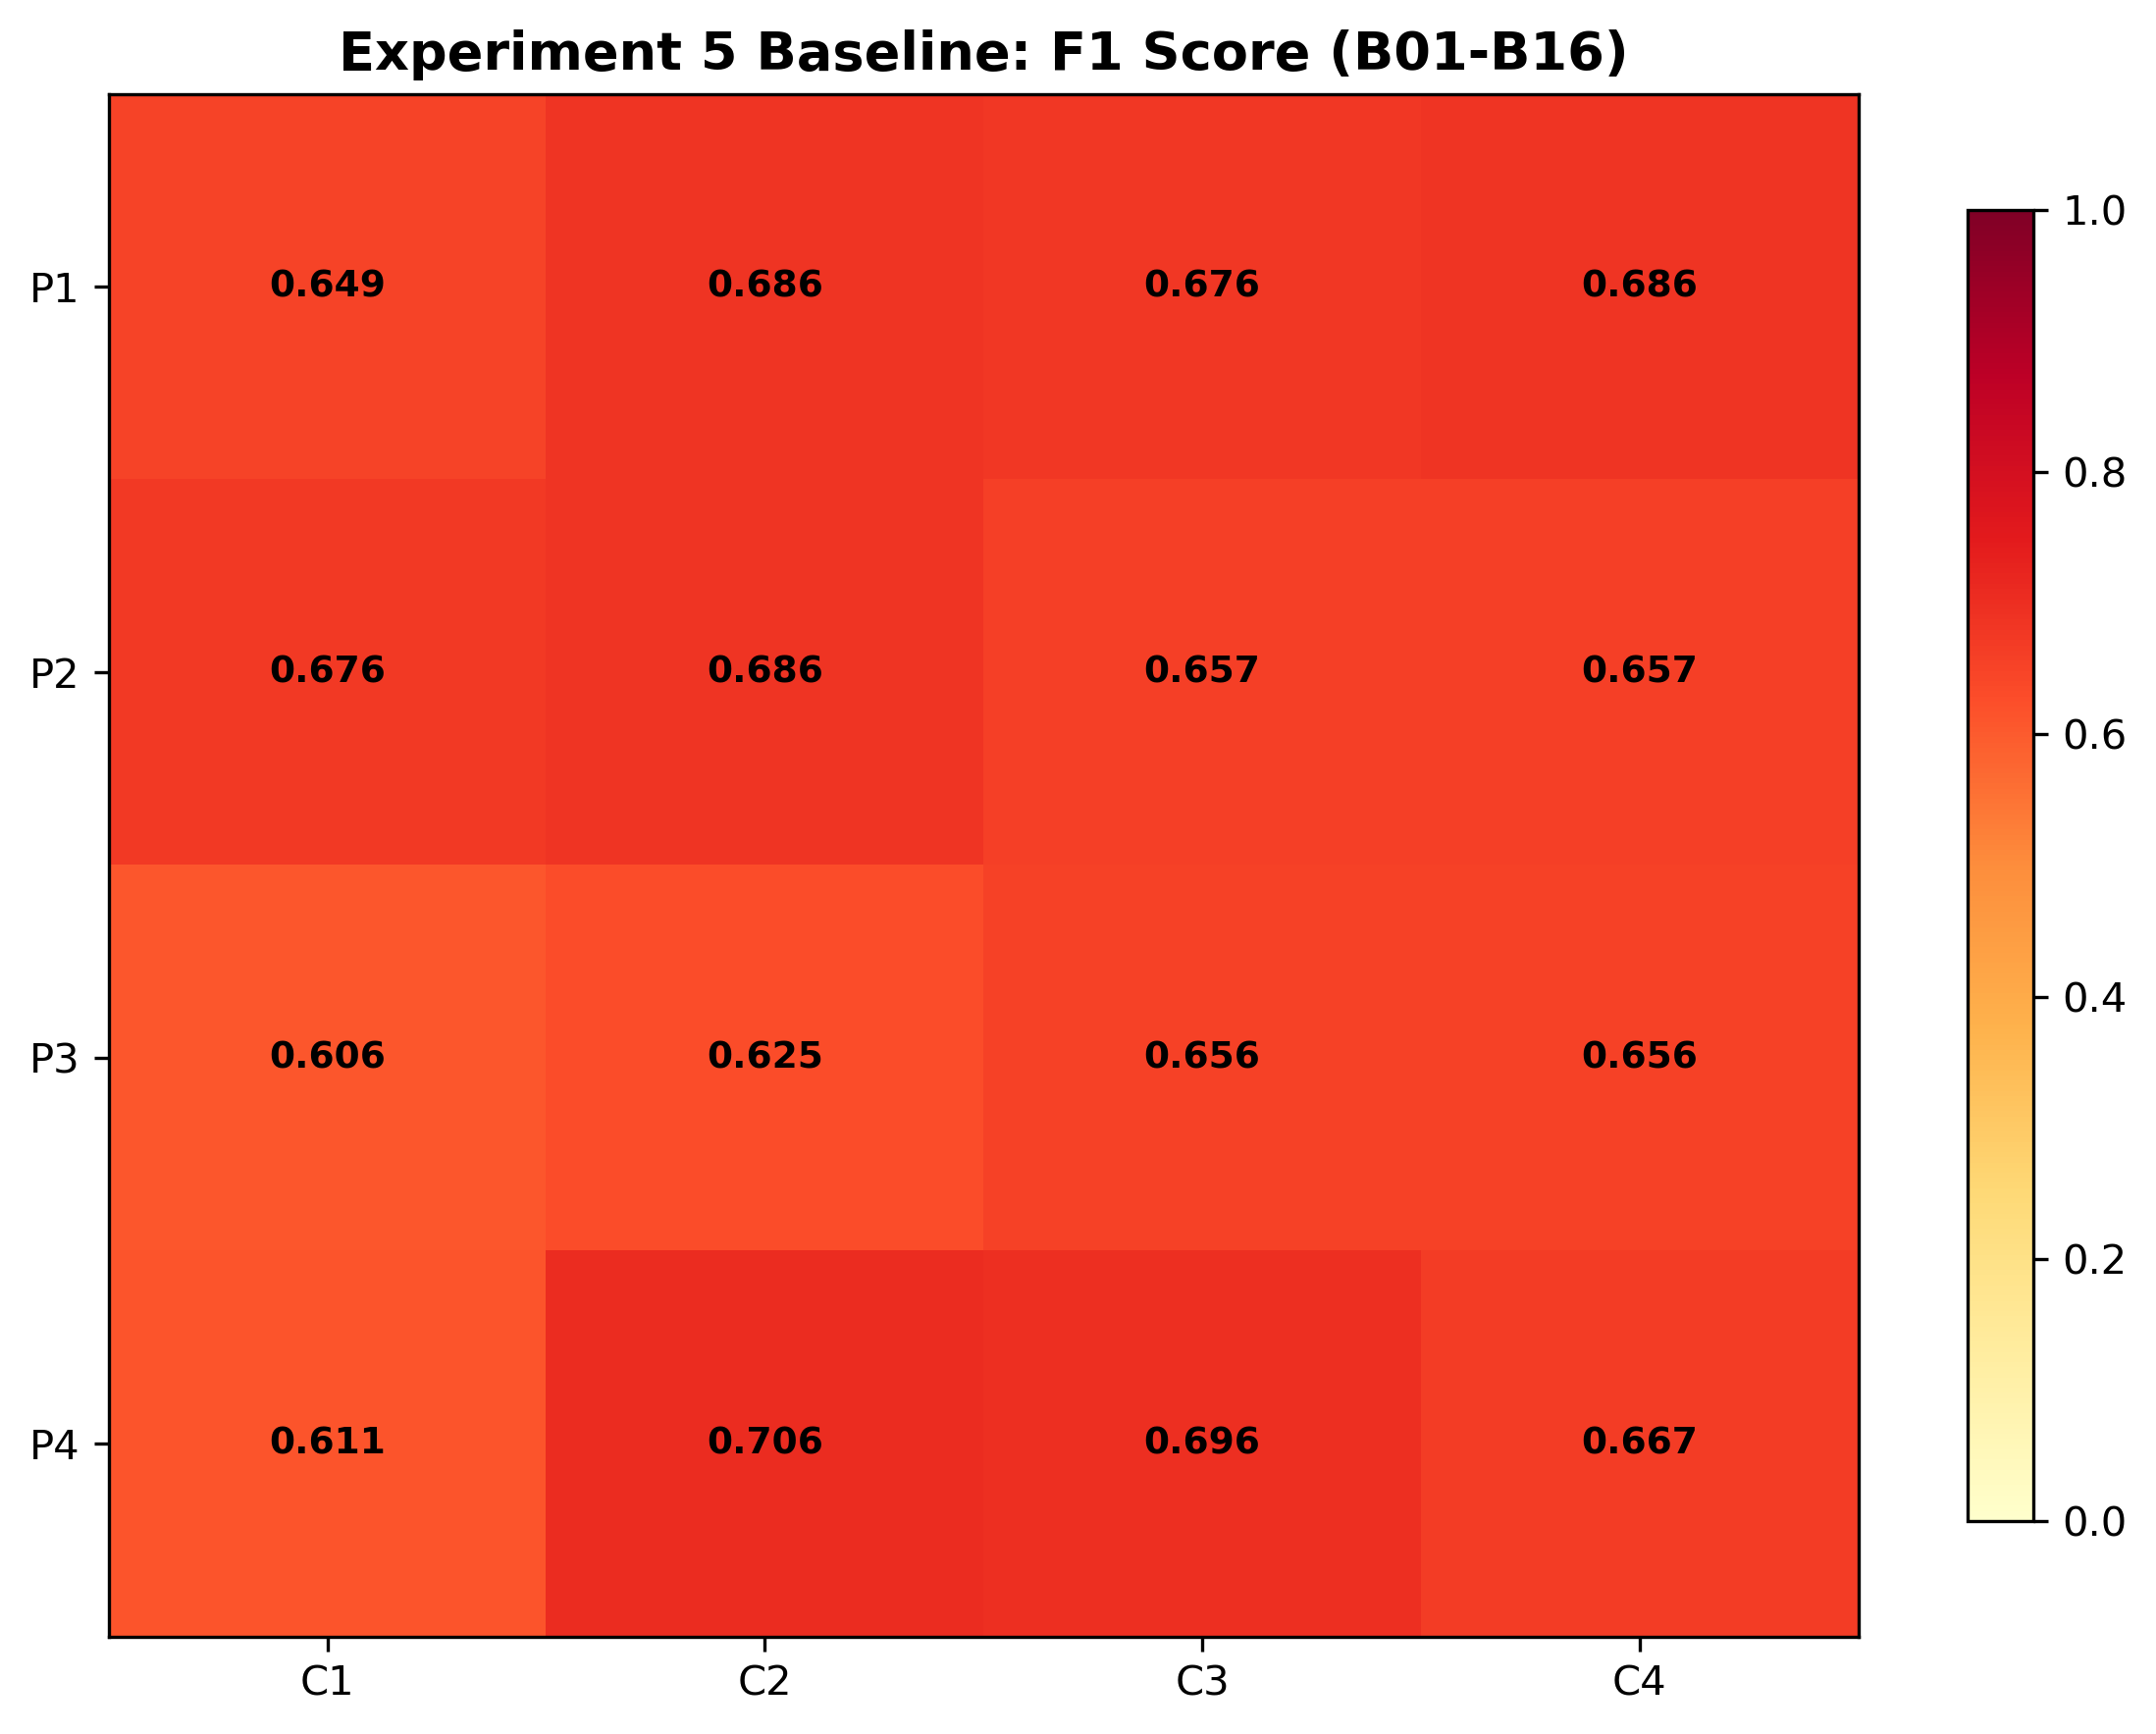
\includegraphics[width=\textwidth]{../figures/exp5_baseline_f1_heatmap.png}
    \caption{实验五 B01--B16 F1 Heatmap}
\end{subfigure}
\hfill
\begin{subfigure}{0.48\textwidth}
    \centering
    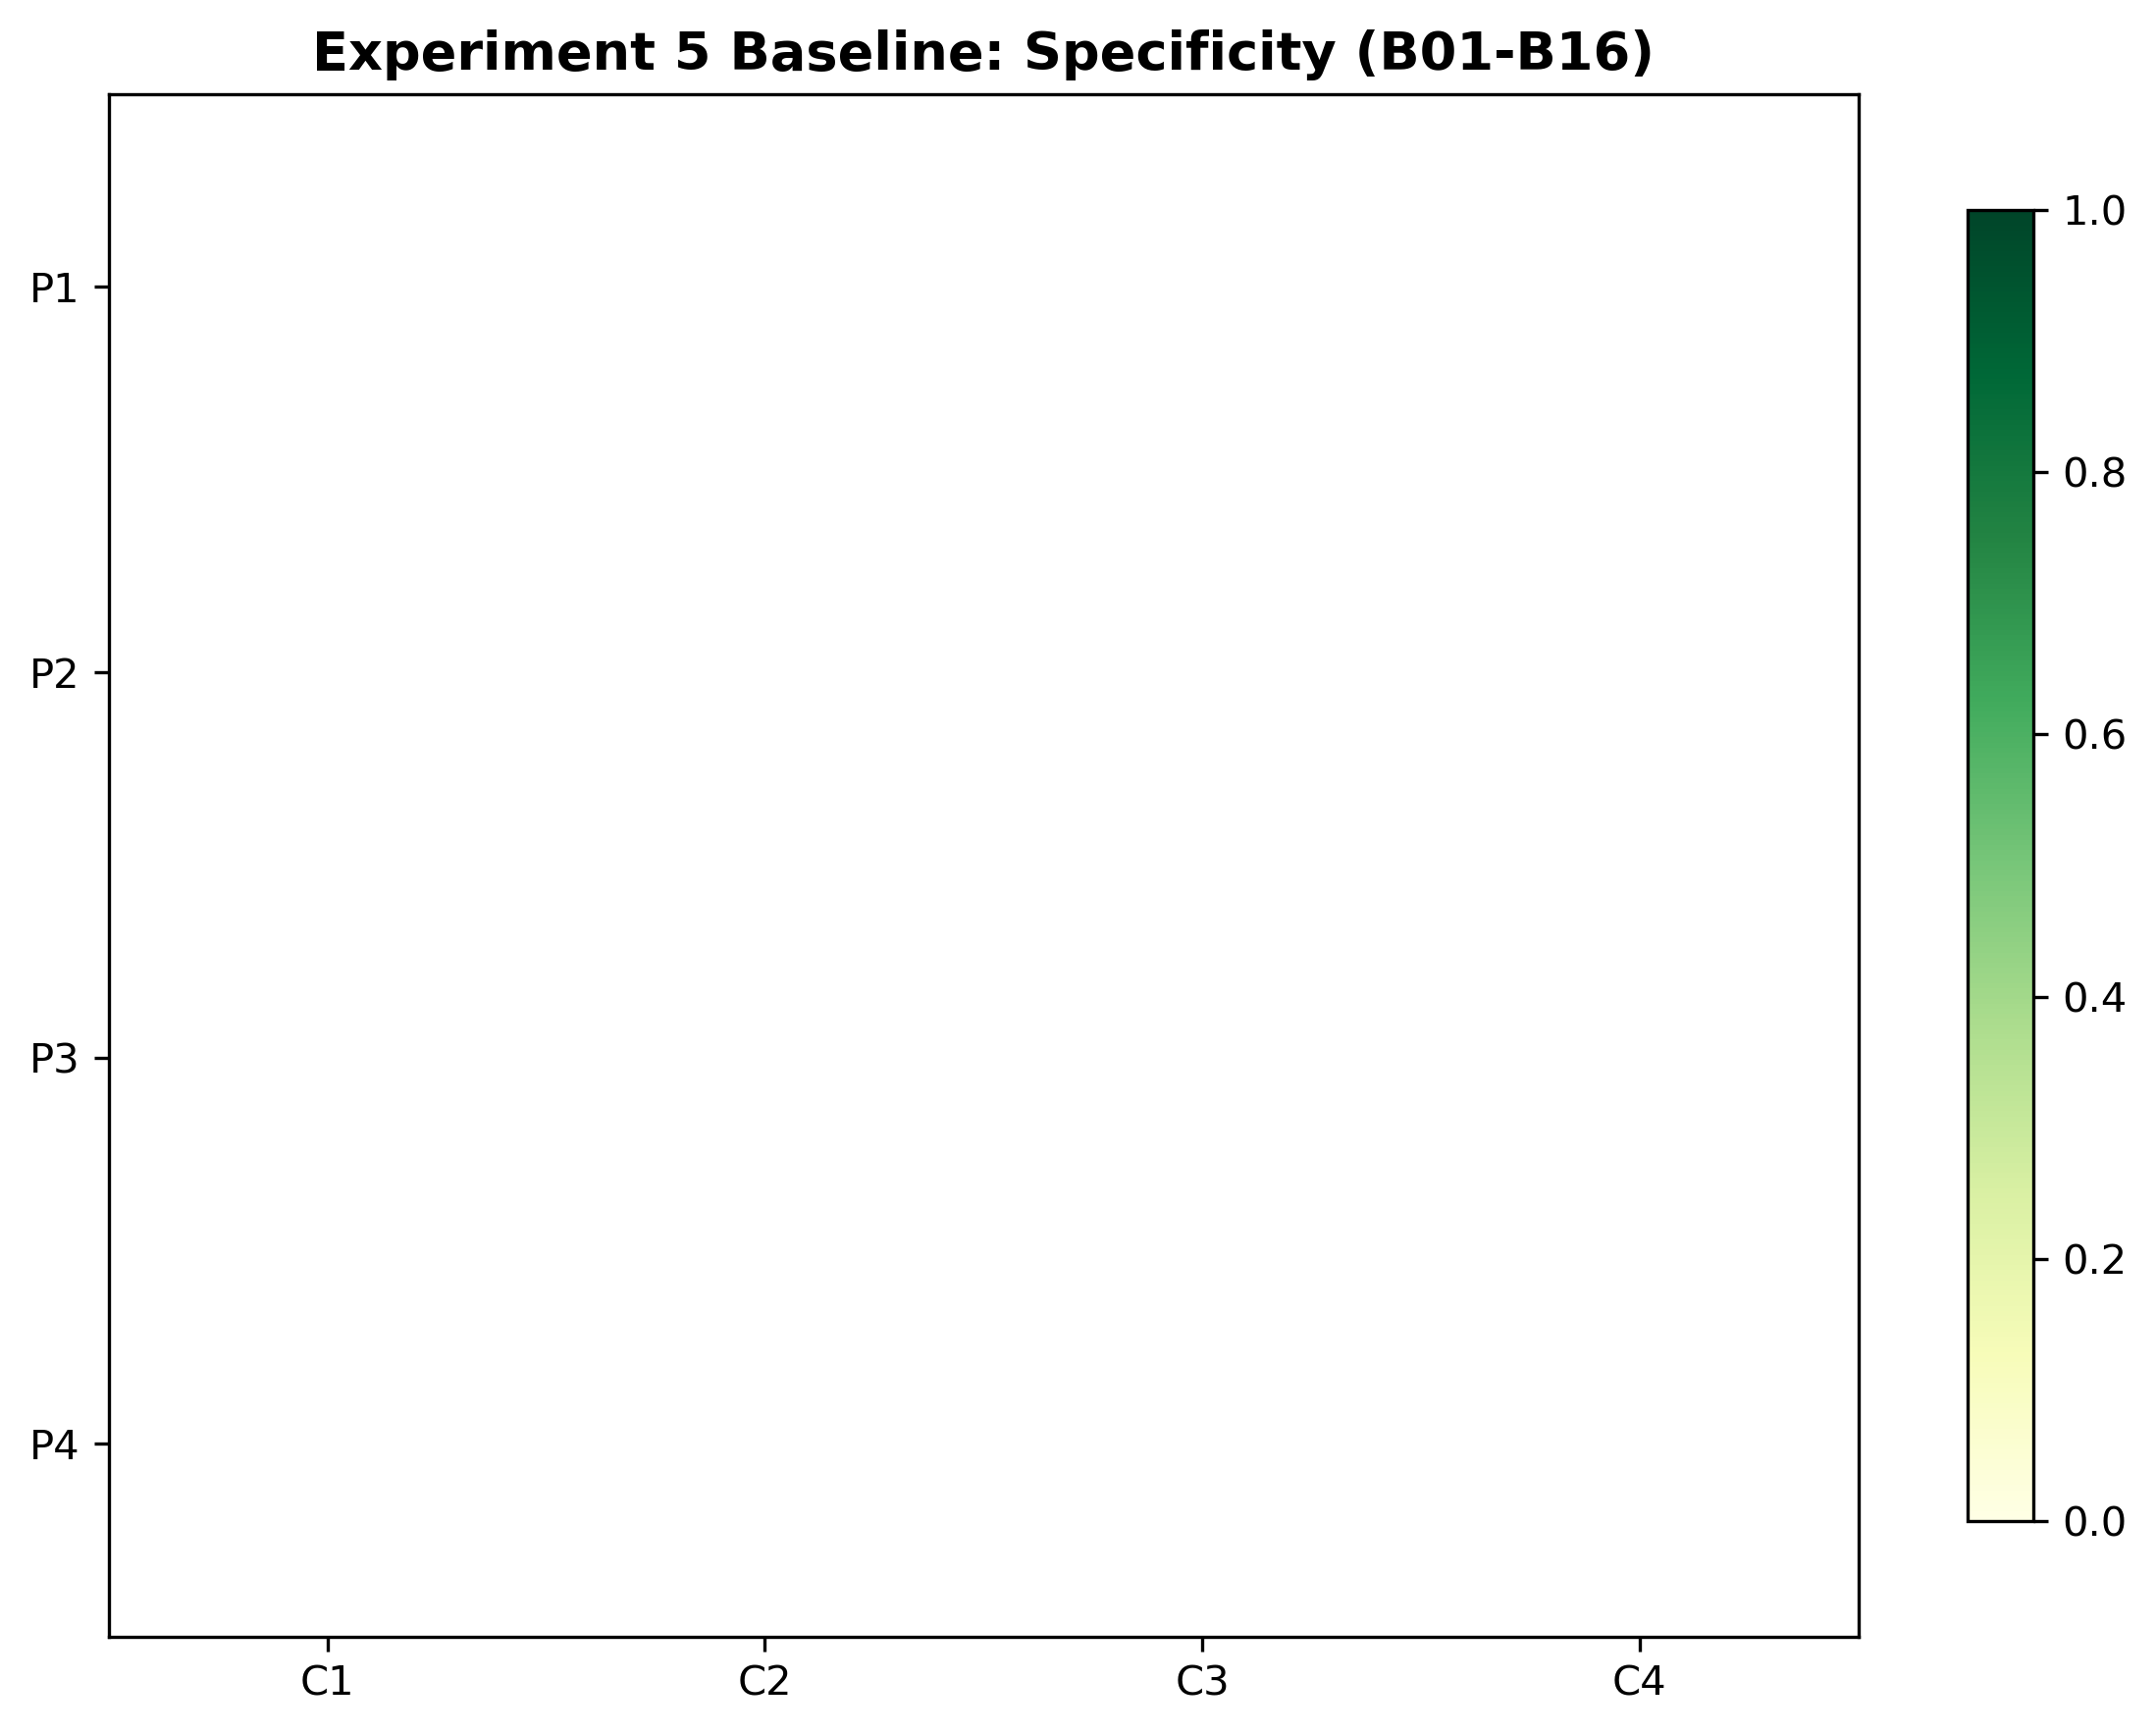
\includegraphics[width=\textwidth]{../figures/exp5_baseline_specificity_heatmap.png}
    \caption{实验五 B01--B16 Specificity Heatmap}
\end{subfigure}
\caption{实验五基线 4$\times$4 Heatmap —— Specificity 普遍极低}
\end{figure}

\begin{figure}[htbp]
\centering
\begin{subfigure}{0.48\textwidth}
    \centering
    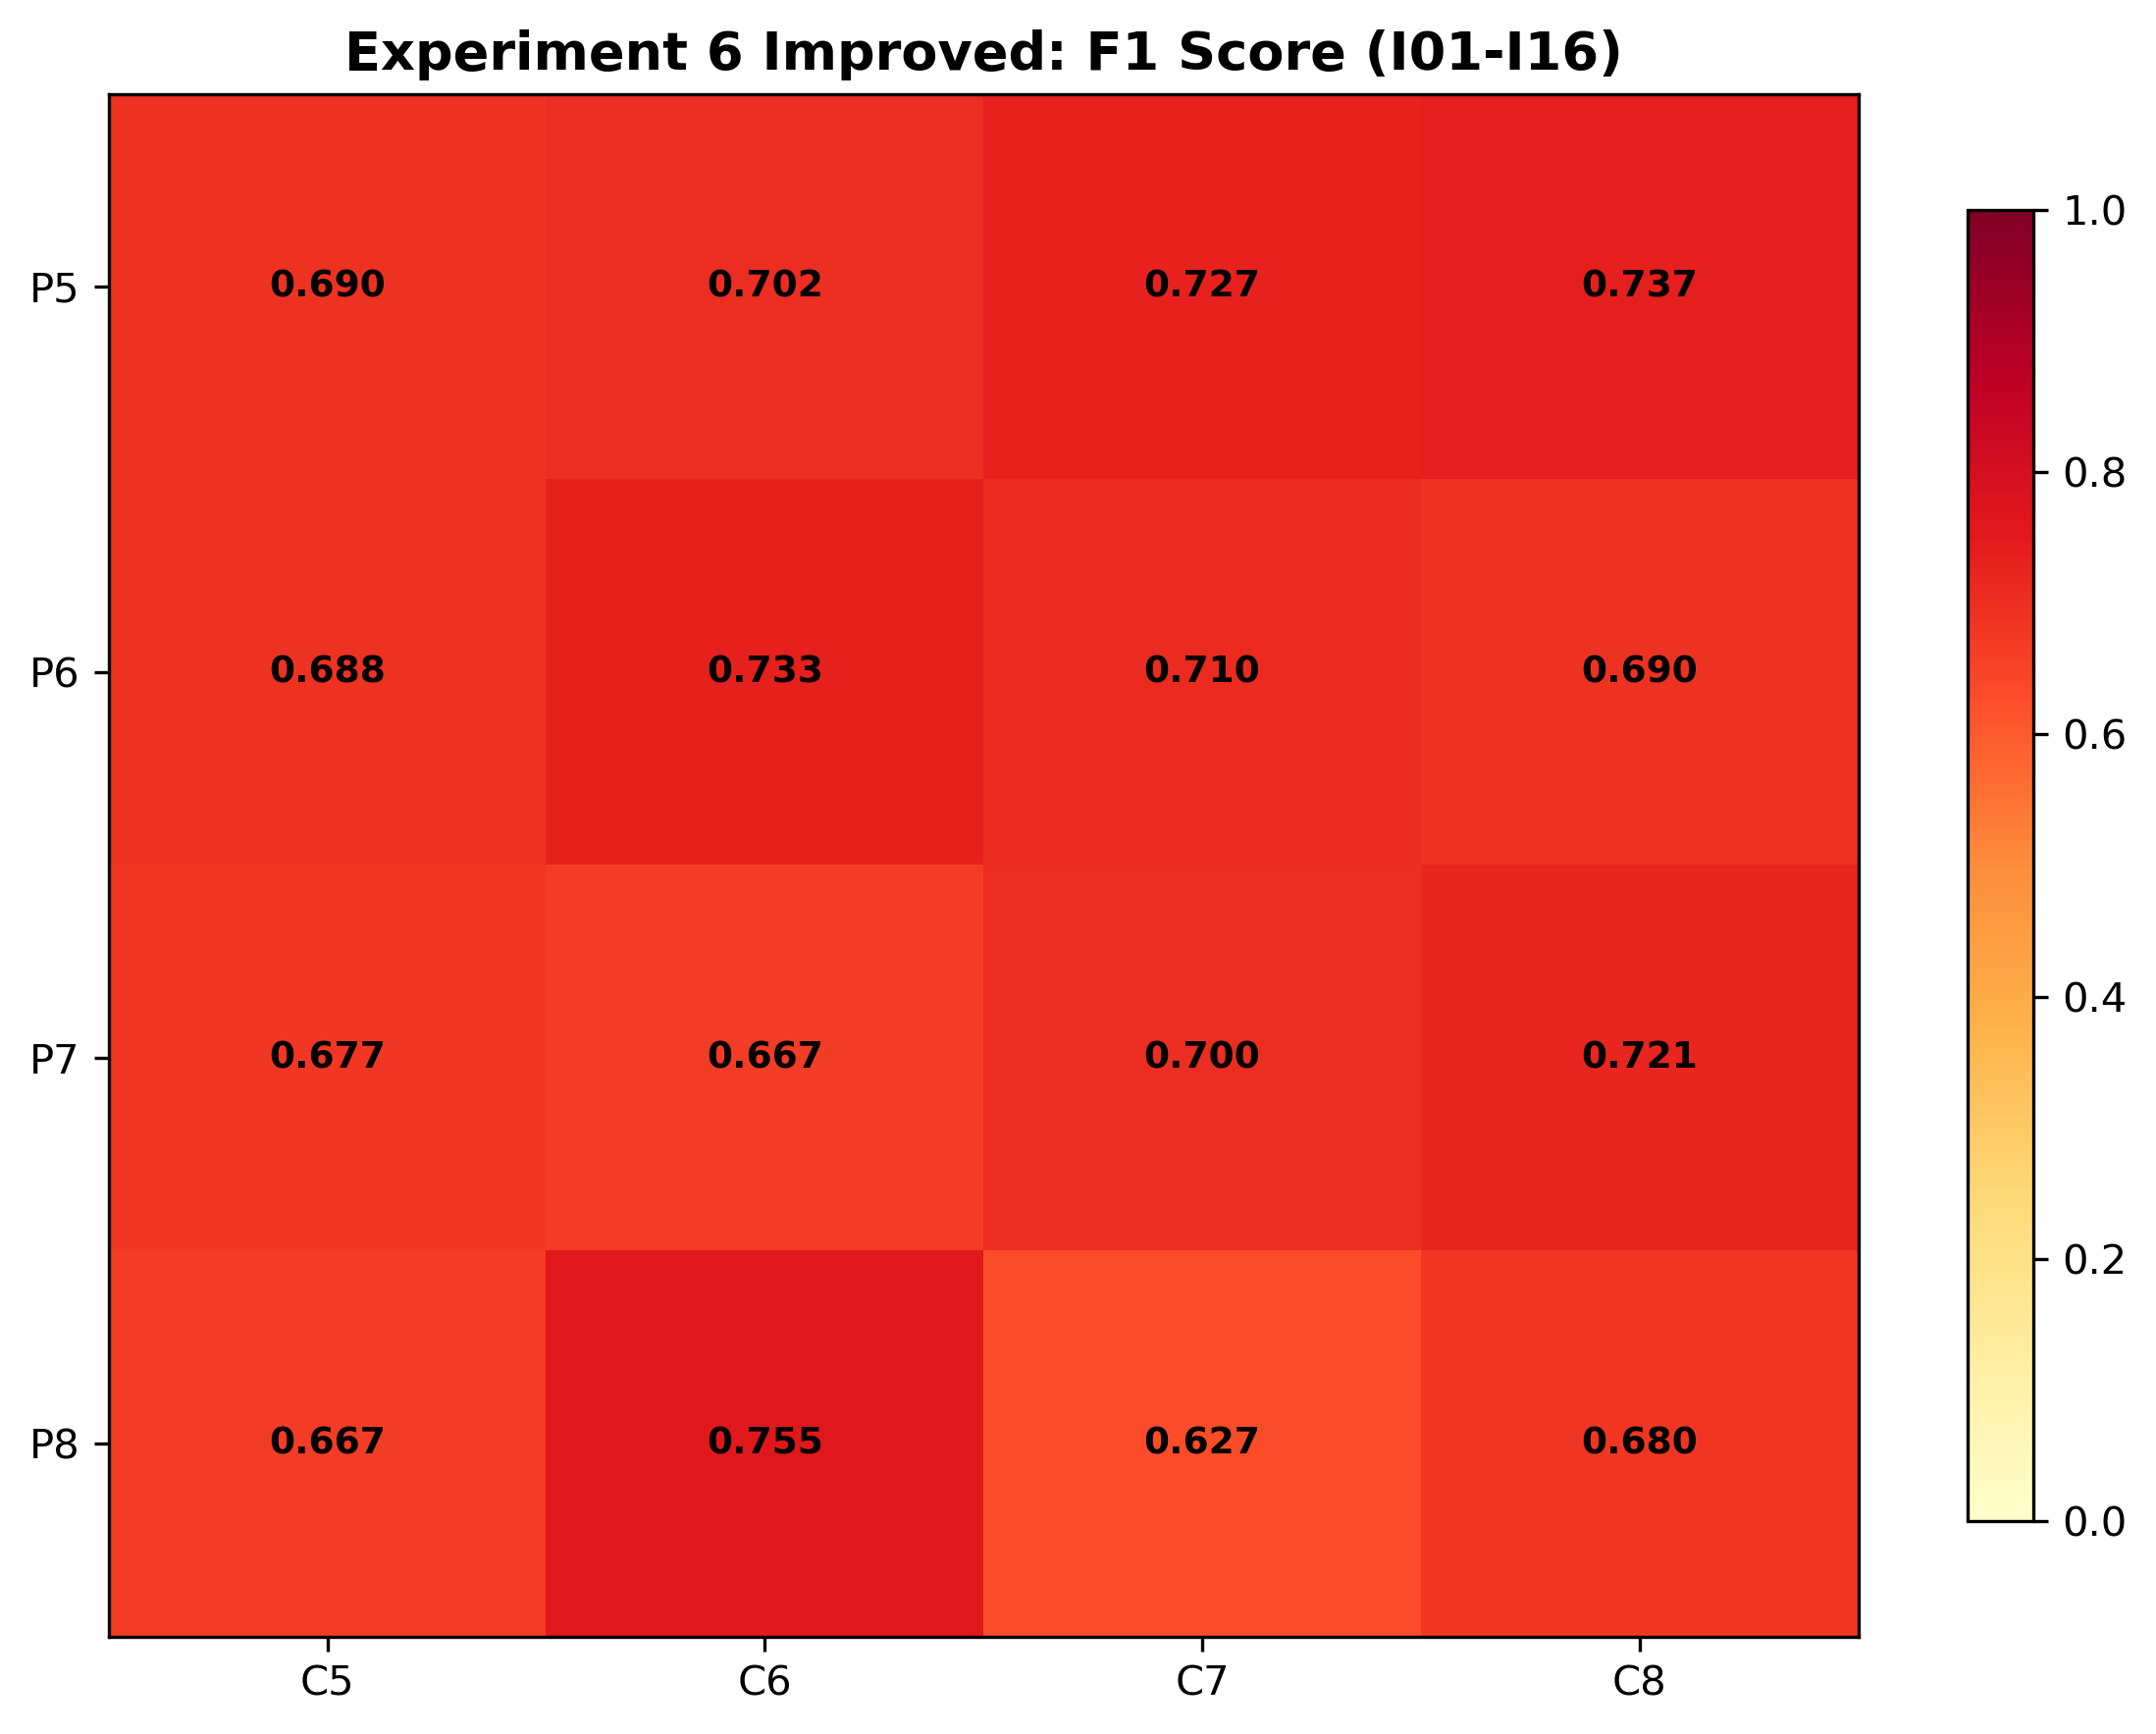
\includegraphics[width=\textwidth]{../figures/exp6_improved_f1_heatmap.png}
    \caption{实验六 I01--I16 F1 Heatmap}
\end{subfigure}
\hfill
\begin{subfigure}{0.48\textwidth}
    \centering
    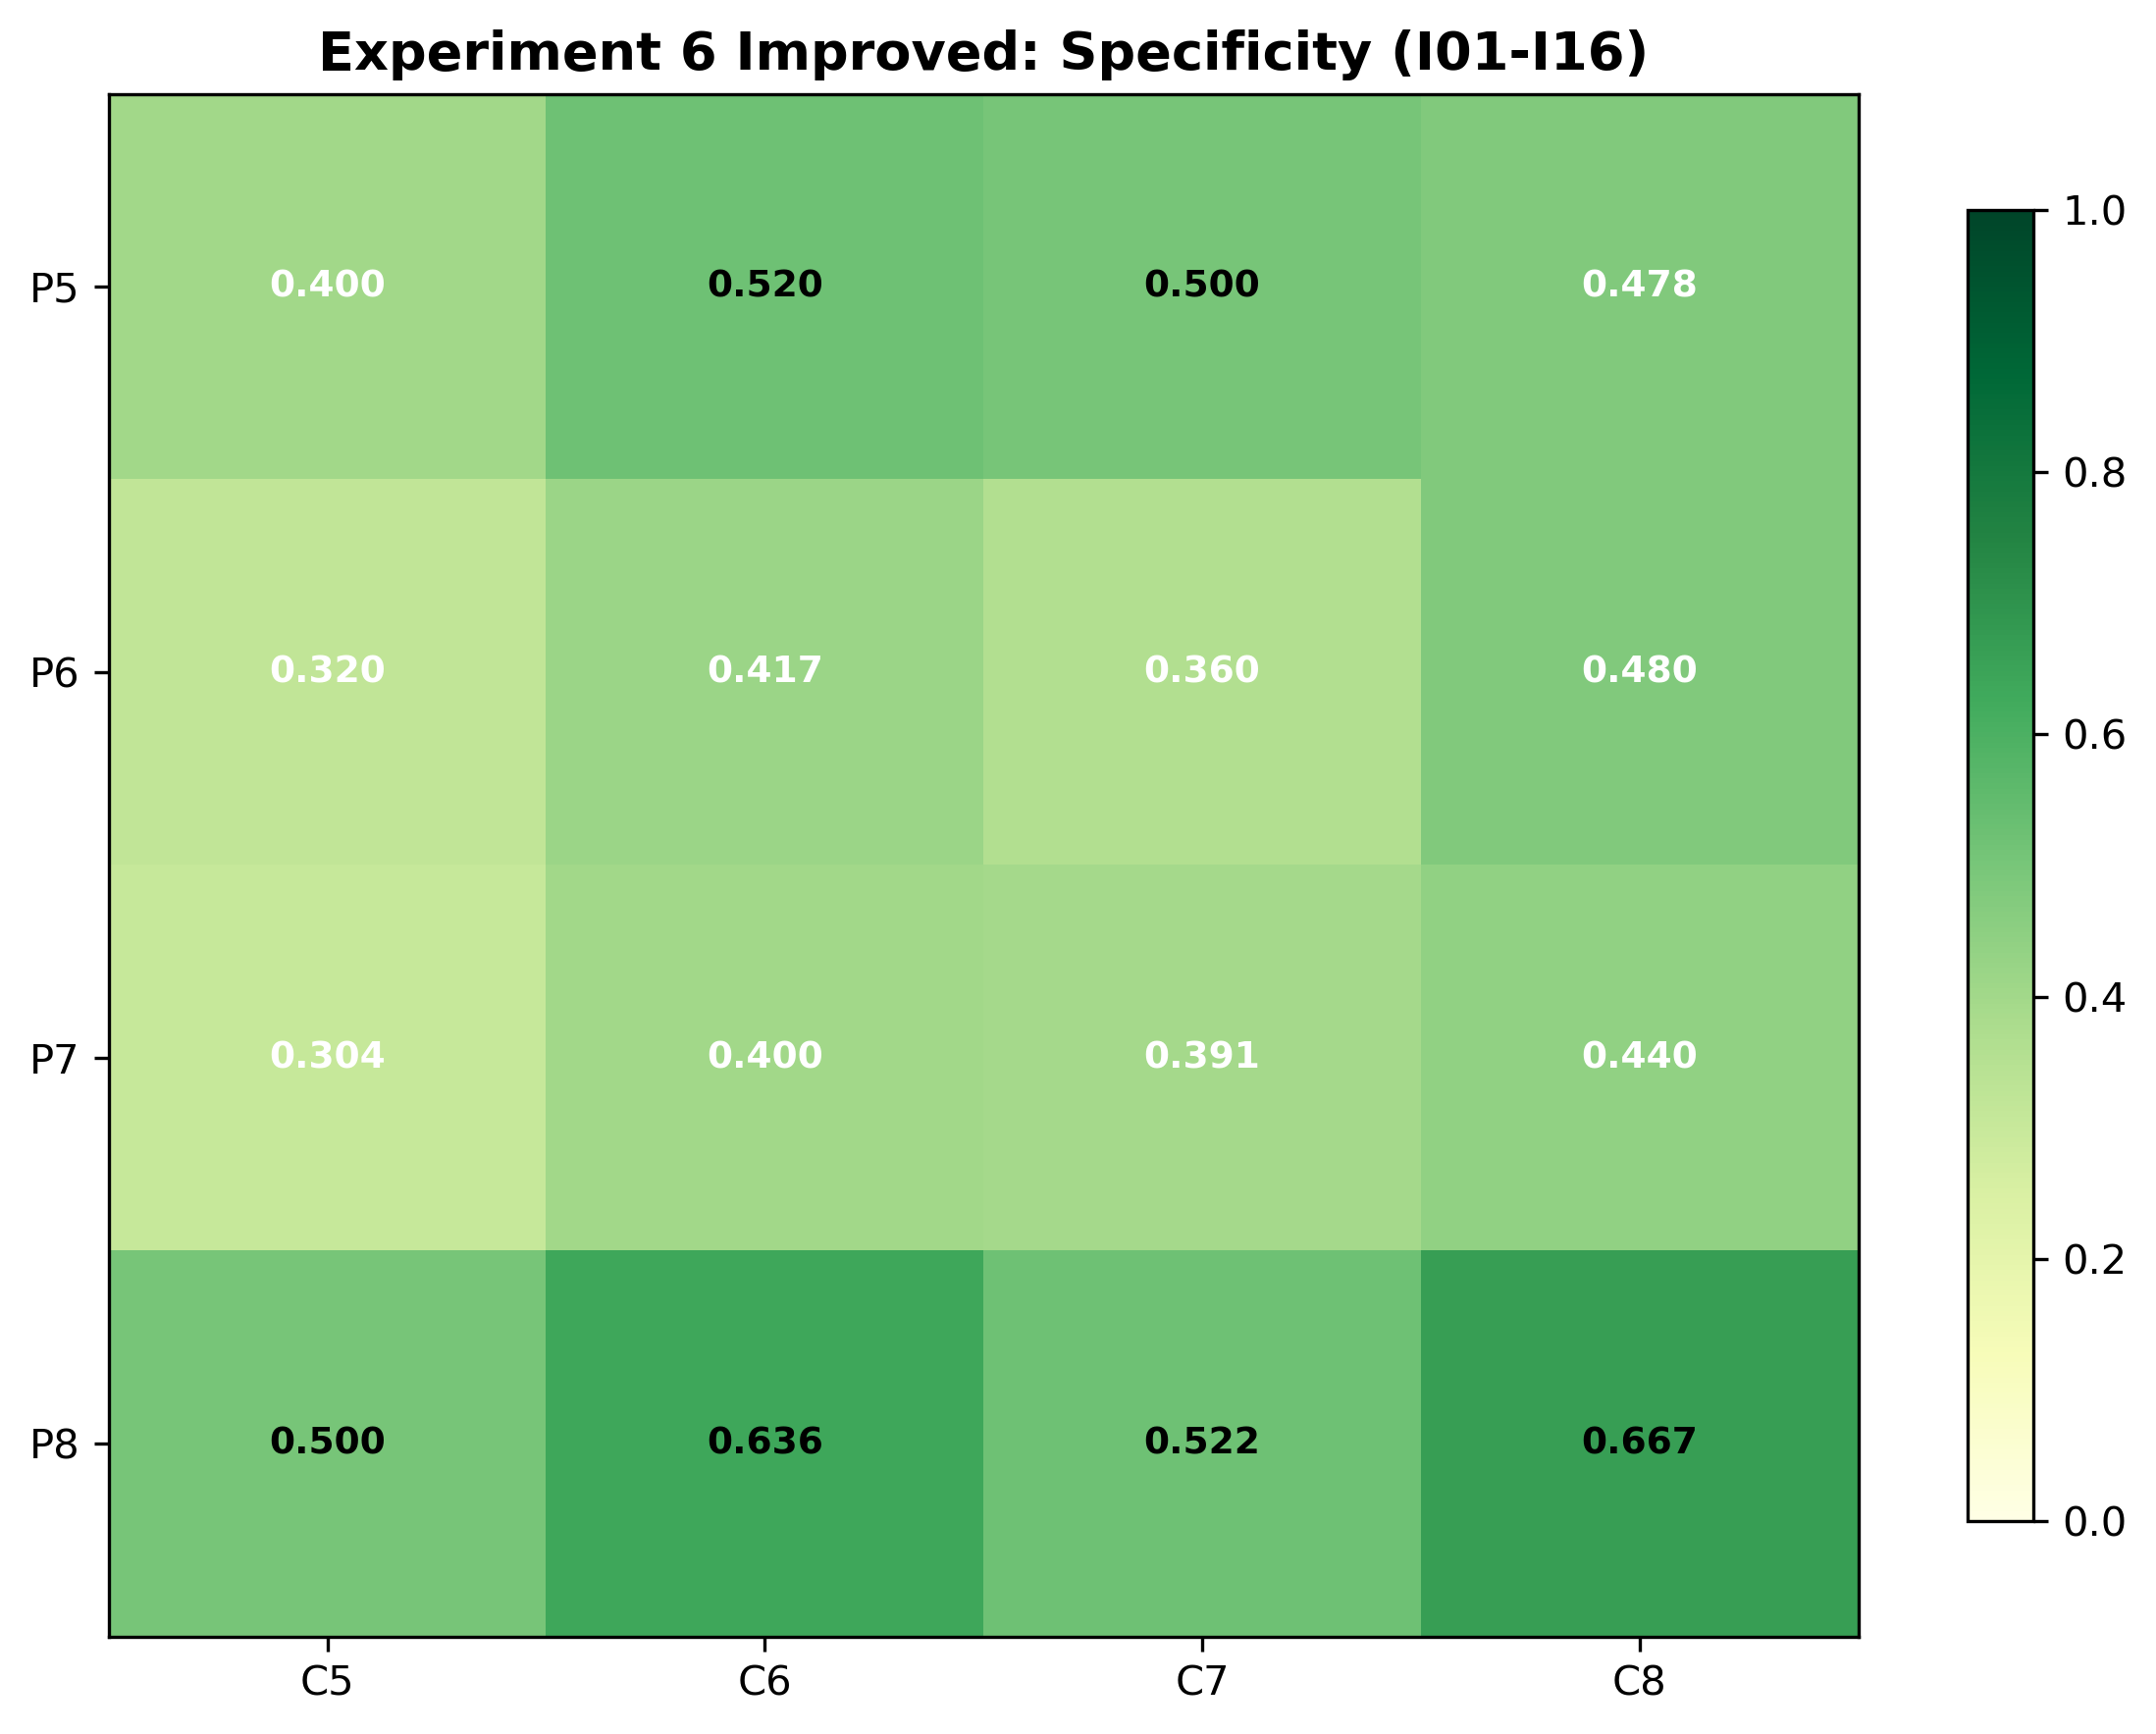
\includegraphics[width=\textwidth]{../figures/exp6_improved_specificity_heatmap.png}
    \caption{实验六 I01--I16 Specificity Heatmap}
\end{subfigure}
\caption{实验六改进 4$\times$4 Heatmap —— P8 行全面优于基线}
\end{figure}

\subsection{B01--B16 vs I01--I16 关键对比}

\begin{table}[htbp]
\centering
\caption{实验五最佳 vs 实验六最佳（同一批 50 条样本）}
\begin{tabular}{lcccccc}
\toprule
对比维度 & 实验五最佳 & 值 & 实验六最佳 & 值 & 提升 \\
\midrule
最佳 F1 & B14 (P4+C2) & 0.7059 & I14 (P8+C6) & 0.7547 & +6.9\% \\
最佳 AUC & B04 (P1+C4) & 0.6352 & I07 (P6+C7) & 0.7358 & +15.8\% \\
最佳 Specificity & B12 (P3+C4) & 0.3600 & I16 (P8+C8) & 0.6667 & +85.2\% \\
最低 FPR & B12 (P3+C4) & 0.6400 & I16 (P8+C8) & 0.3333 & $-$48.0\% \\
最佳 BalAcc & B12 (P3+C4) & $\sim$0.58 & I14 (P8+C6) & 0.7182 & +23.8\% \\
\bottomrule
\end{tabular}
\end{table}

\textbf{核心发现：}
\begin{enumerate}
    \item \textbf{全部关键指标被刷新}：I01--I16 在 F1、AUC、Specificity、FPR、Balanced Accuracy 五个维度全面超越 B01--B16 最佳值。
    \item \textbf{P8 (Strict Maintainer) 是最有效的 Prompt}：I13--I16（P8行）的 Specificity 均值 0.581，远超其他 Prompt 行（P5: 0.475, P6: 0.394, P7: 0.384）。P8 的角色锚定和硬规则从根本上改变了模型的输出分布。
    \item \textbf{I14 综合最优}：F1=0.7547（超 B14 的 0.7059）\textit{同时} Specificity=0.6364（接近 B12 的 2 倍）。这是实验六中唯一在 F1 和 Specificity 上同时大幅领先的组。
    \item \textbf{I16 识别 unmerged 最强}：Specificity=0.6667，FPR 仅 0.3333，意味着仅 1/3 的真实 unmerged PR 被误判为 merged（实验五约为 3/4）。
    \item \textbf{C7 (Historical PR) 提升 AUC 最明显}：I03 (AUC=0.7264)、I07 (AUC=0.7358)、I11 (AUC=0.7087) —— 含 C7 的组合 AUC 均值最高，说明历史相似 PR 提供了有价值的判别信息。
\end{enumerate}

\subsection{Review Comment Generation 质量}

\begin{table}[htbp]
\centering
\caption{主实验中最佳改进组合的评论质量}
\begin{tabular}{lccccc}
\toprule
方法 & Risk Coverage & Actionability & Specificity & Blocker+Major & Avg Comments/PR \\
\midrule
I14 (P8+C6) & \textbf{1.000} & \textbf{0.930} & 0.390 & 41.8\% & 4.6 \\
I16 (P8+C8) & 0.977 & 0.928 & \textbf{0.486} & \textbf{51.0\%} & 5.4 \\
\bottomrule
\end{tabular}
\end{table}

P8 生成的评论质量与分类改进方向一致：
\begin{itemize}
    \item I14 的 Risk Coverage 为 1.000，Actionability 为 0.930，说明风险清单和严格 Prompt 能转化为可执行建议。
    \item I16 的 Blocker+Major 占比达到 51.0\%，表明模型更倾向指出测试、兼容性和范围等高优先级风险，而不只是输出 style nit。
\end{itemize}

自动文本重合指标 BLEU/ROUGE 整体偏低，说明代码审查意见表达多样，文本重合度不适合作为评论质量的唯一判据。

\begin{figure}[htbp]
\centering
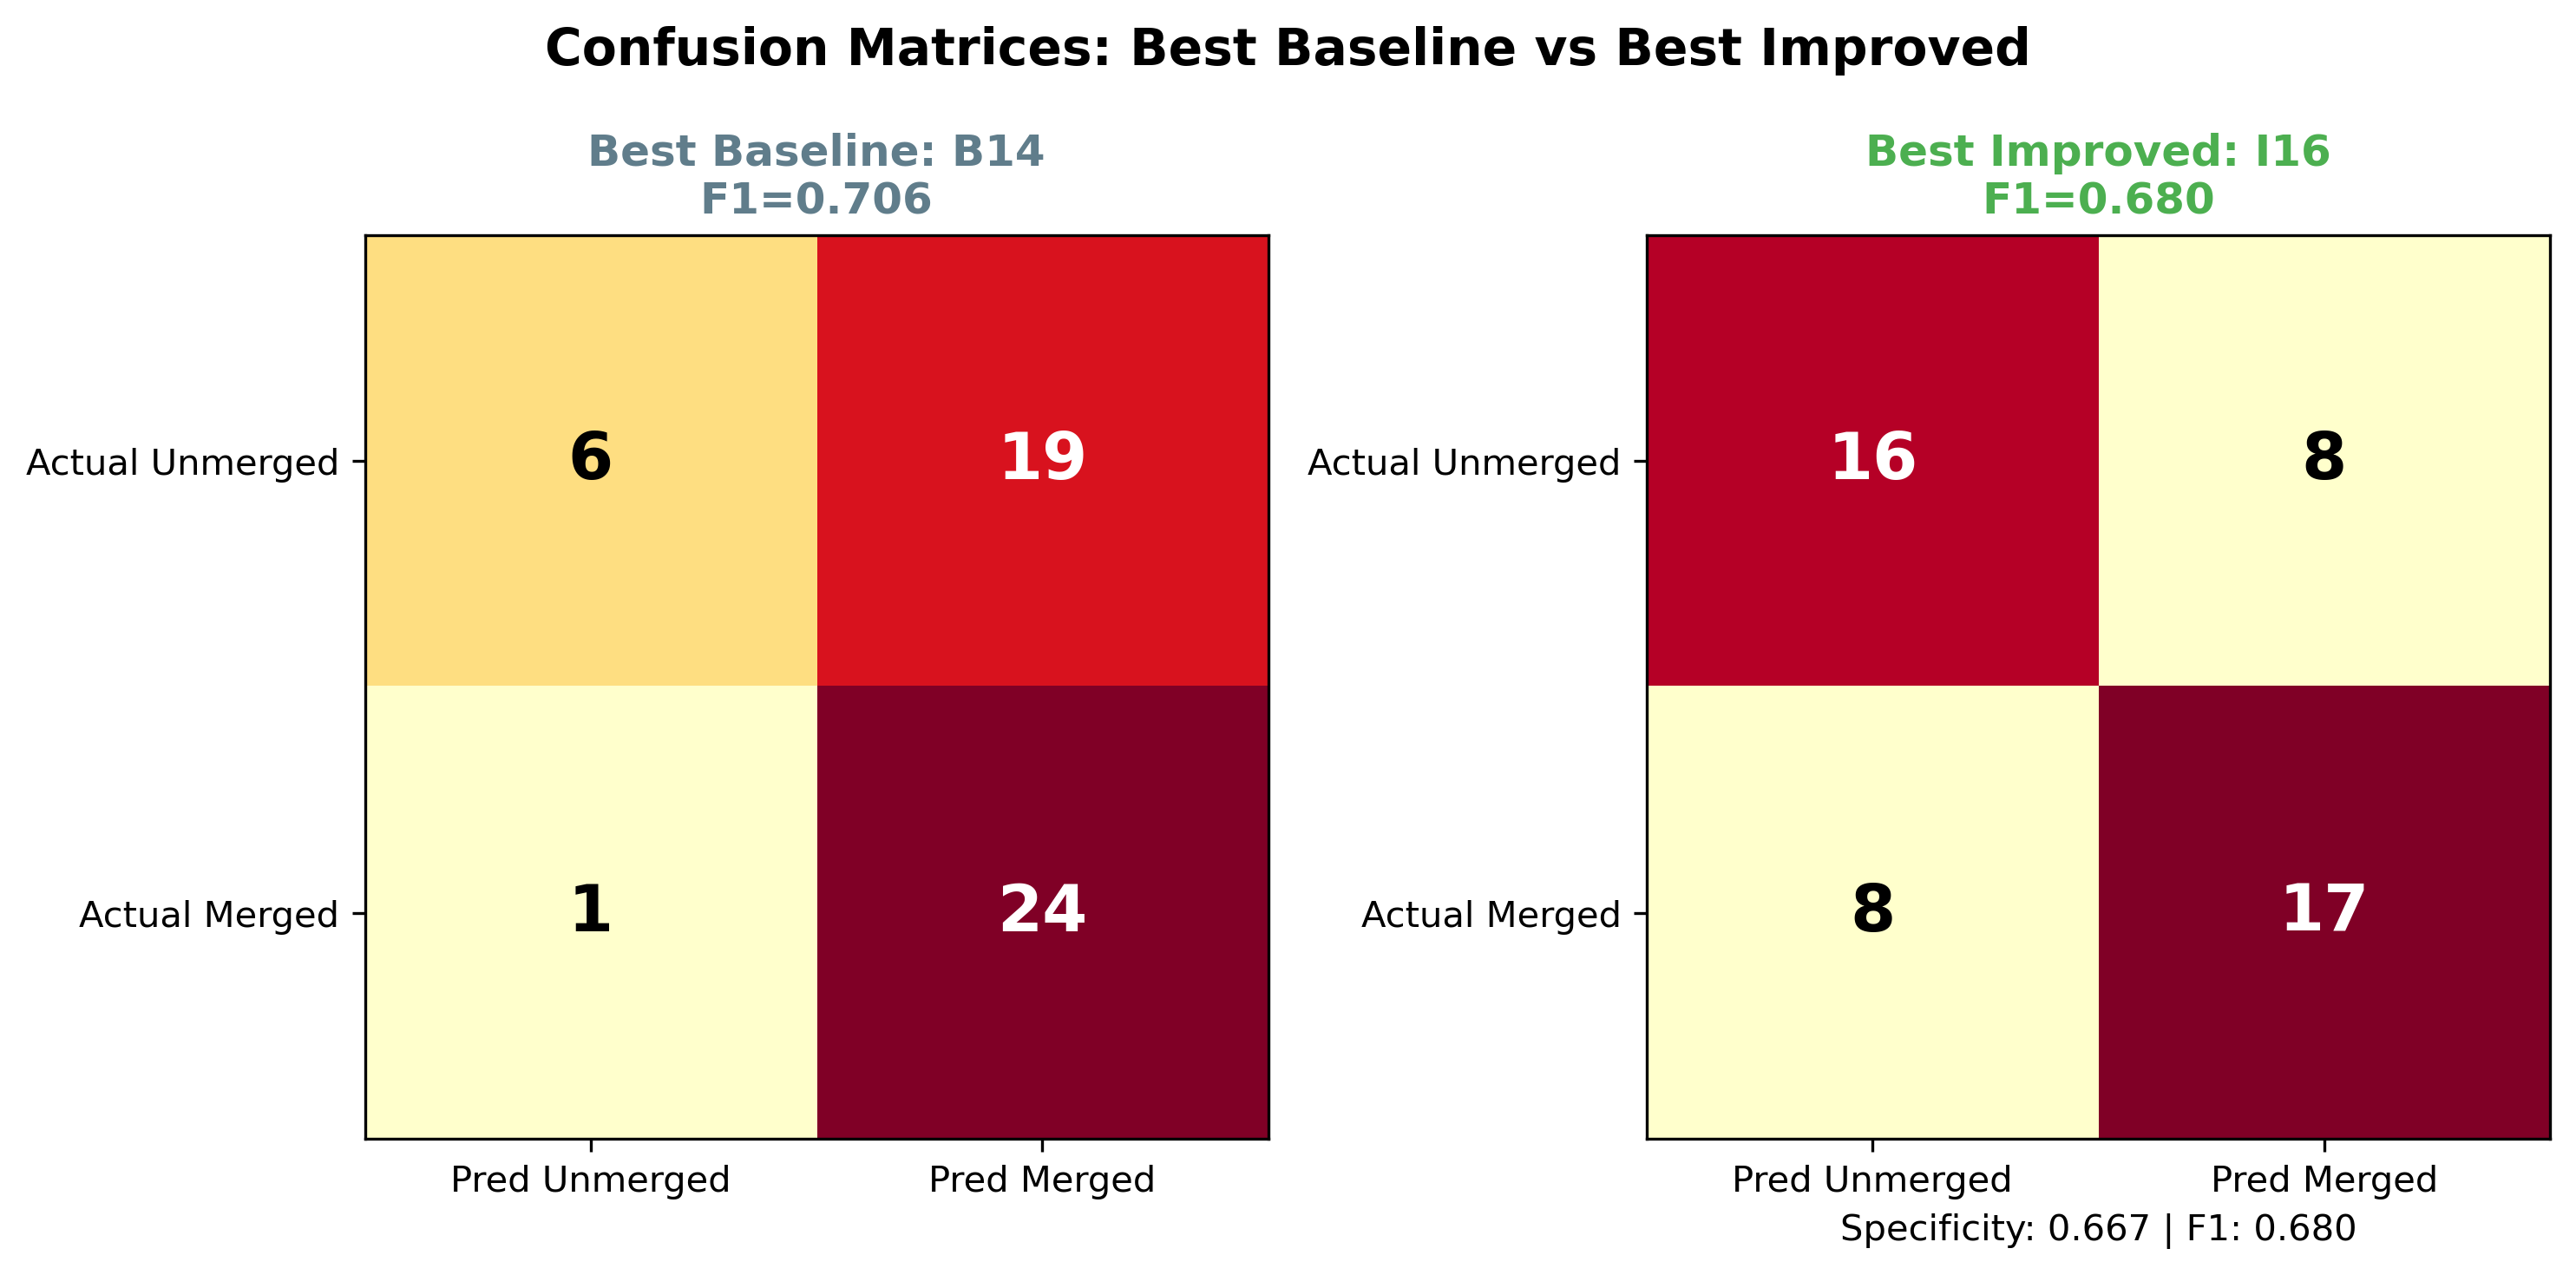
\includegraphics[width=\textwidth]{../figures/best_confusion_matrices.png}
\caption{最佳基线与最佳改进组合的混淆矩阵对比}
\end{figure}

\begin{figure}[htbp]
\centering
\begin{subfigure}{0.48\textwidth}
    \centering
    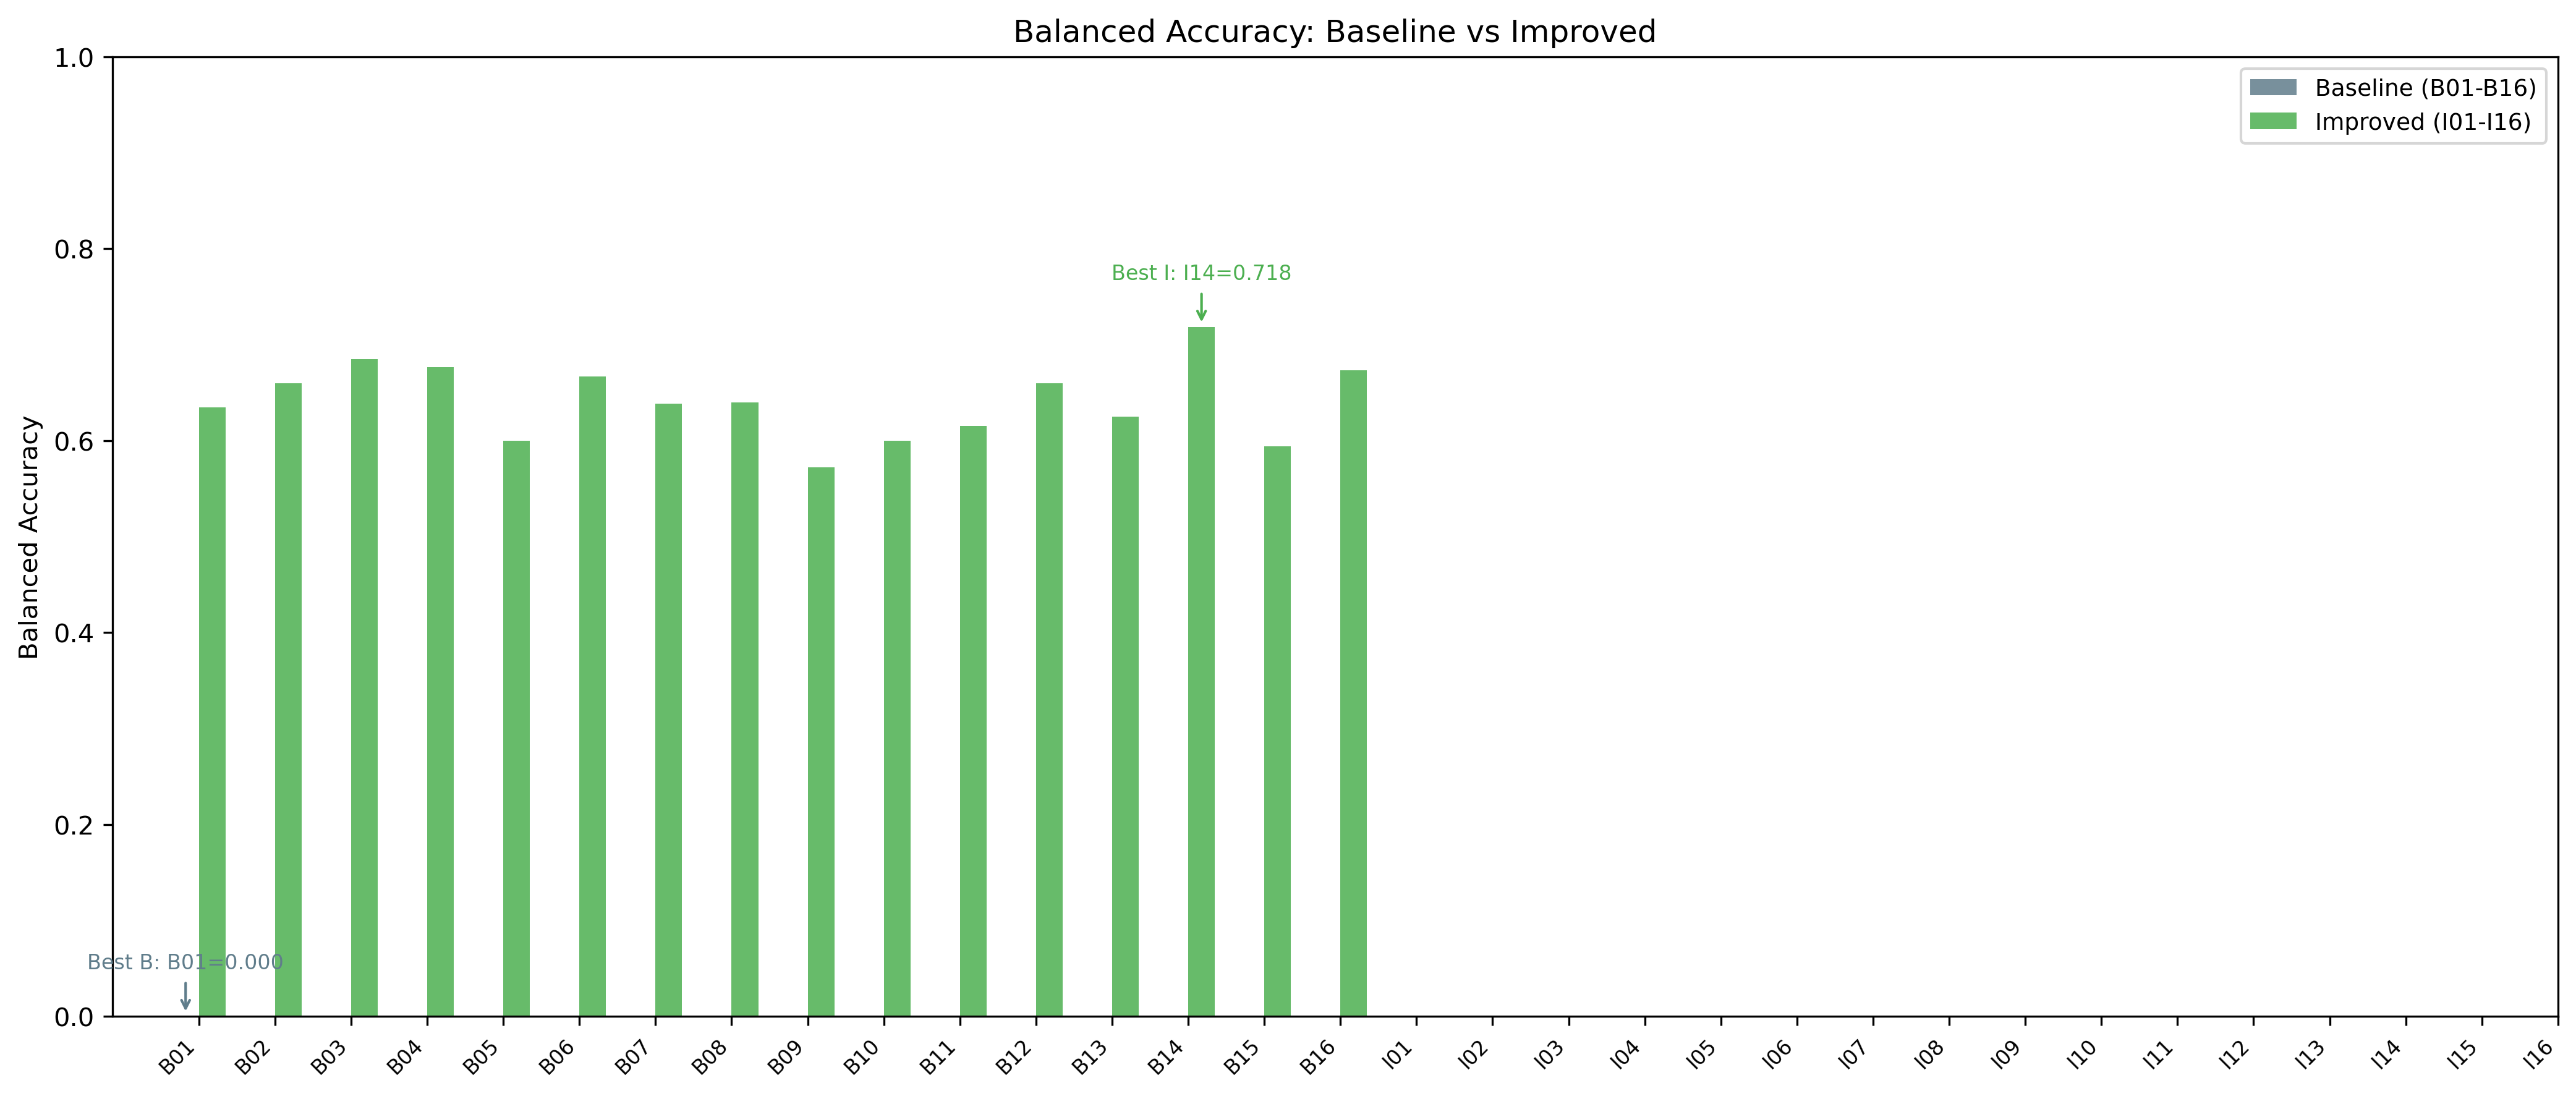
\includegraphics[width=\textwidth]{../figures/baseline_vs_improved_balacc.png}
    \caption{Balanced Accuracy 对比}
\end{subfigure}
\hfill
\begin{subfigure}{0.48\textwidth}
    \centering
    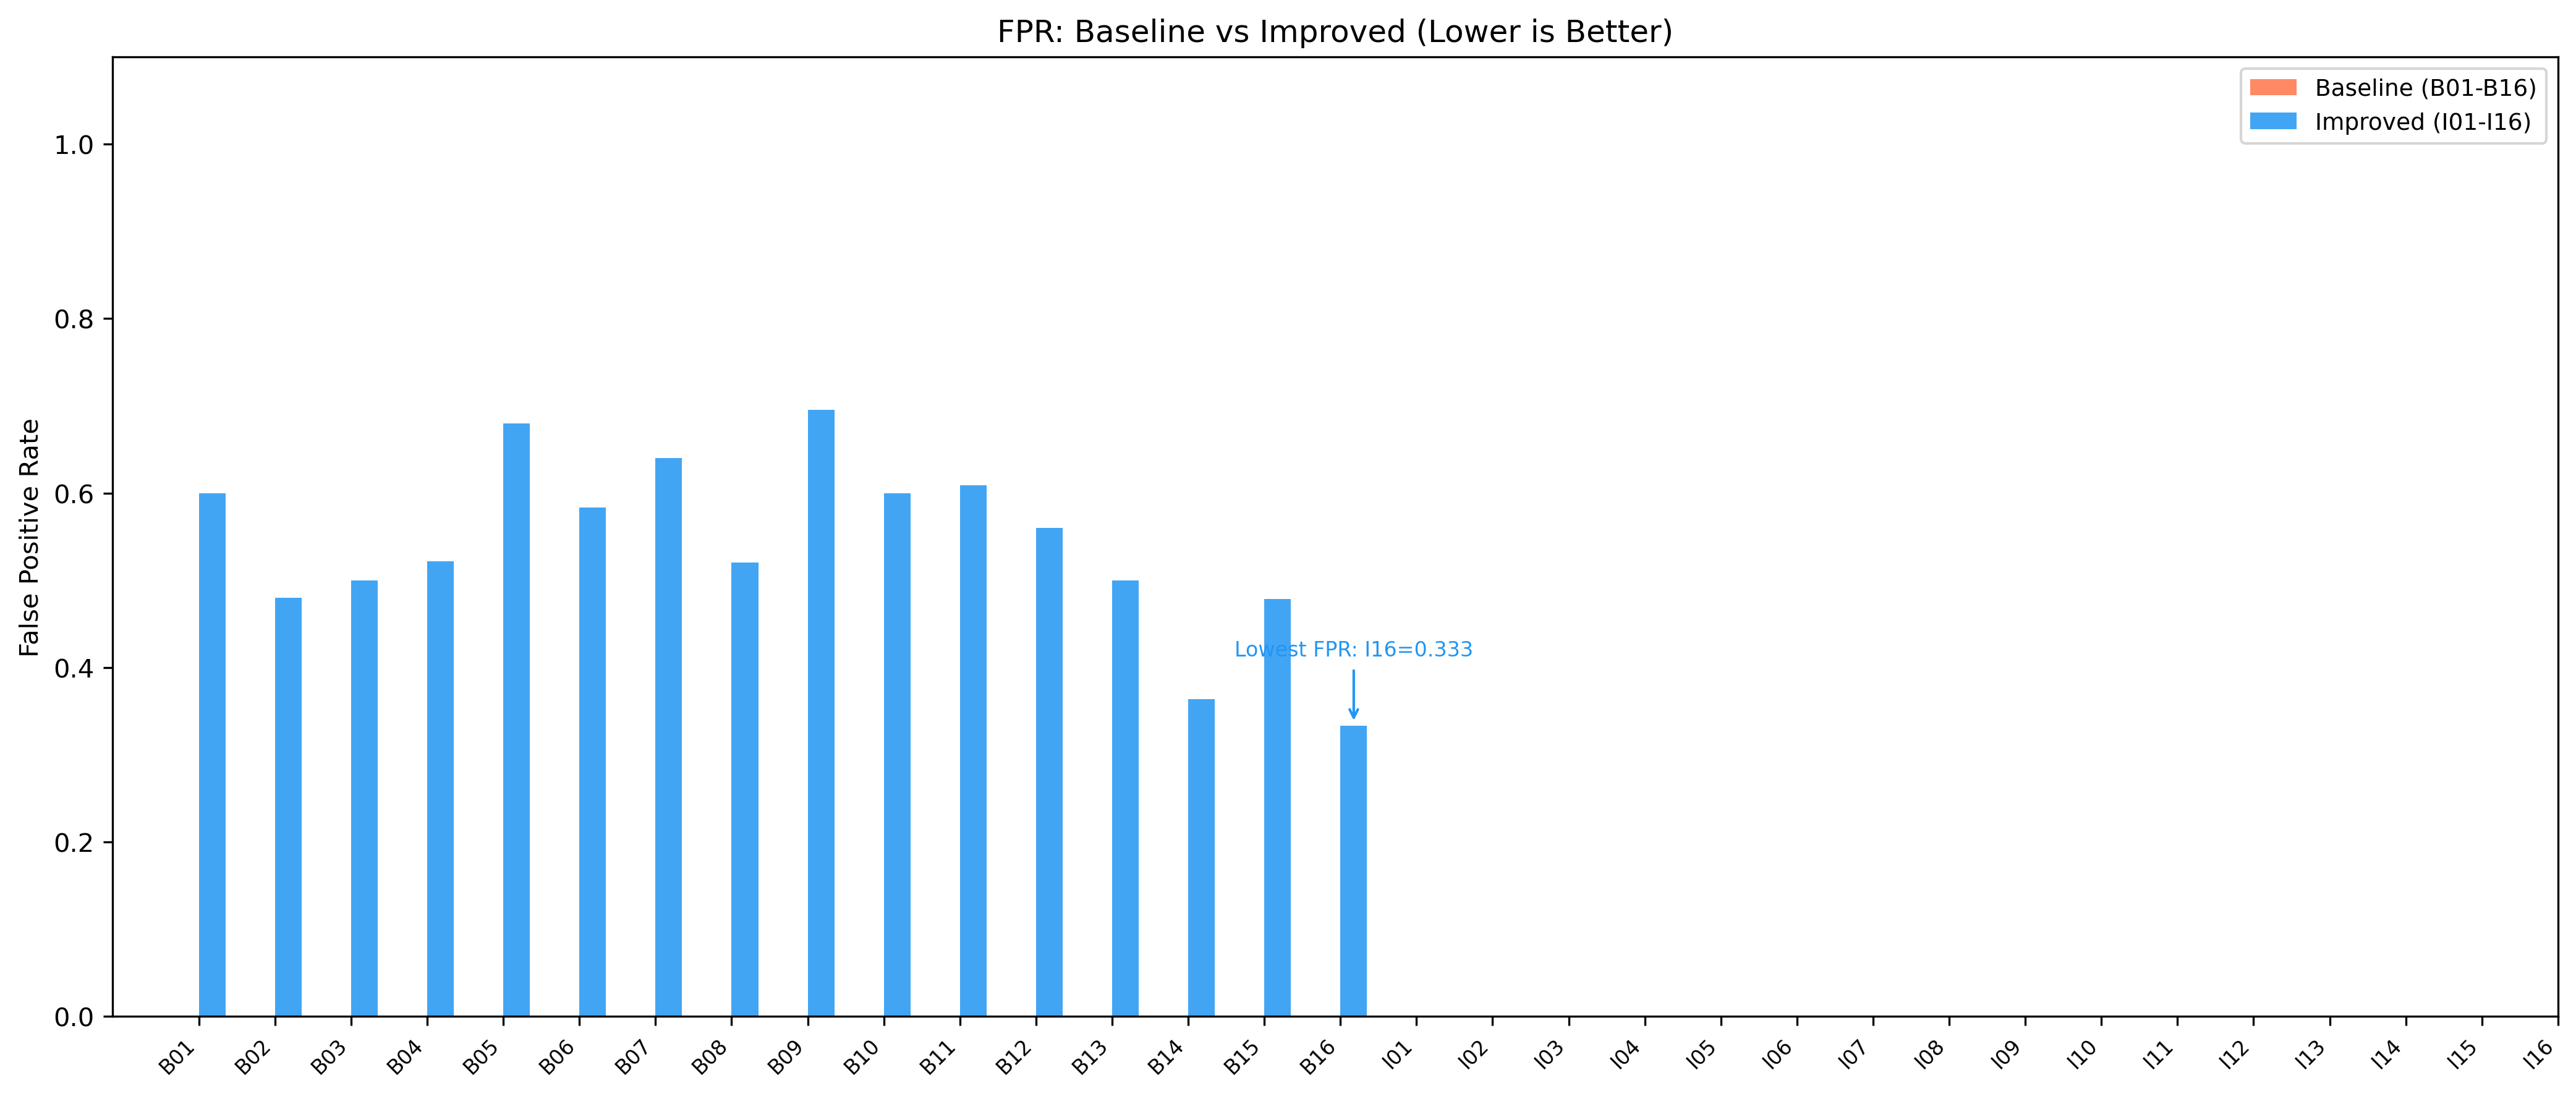
\includegraphics[width=\textwidth]{../figures/baseline_vs_improved_fpr.png}
    \caption{FPR 对比（越低越好）}
\end{subfigure}
\caption{B01--B16 vs I01--I16：Balanced Accuracy 与 FPR 全面对比}
\end{figure}

\begin{figure}[htbp]
\centering
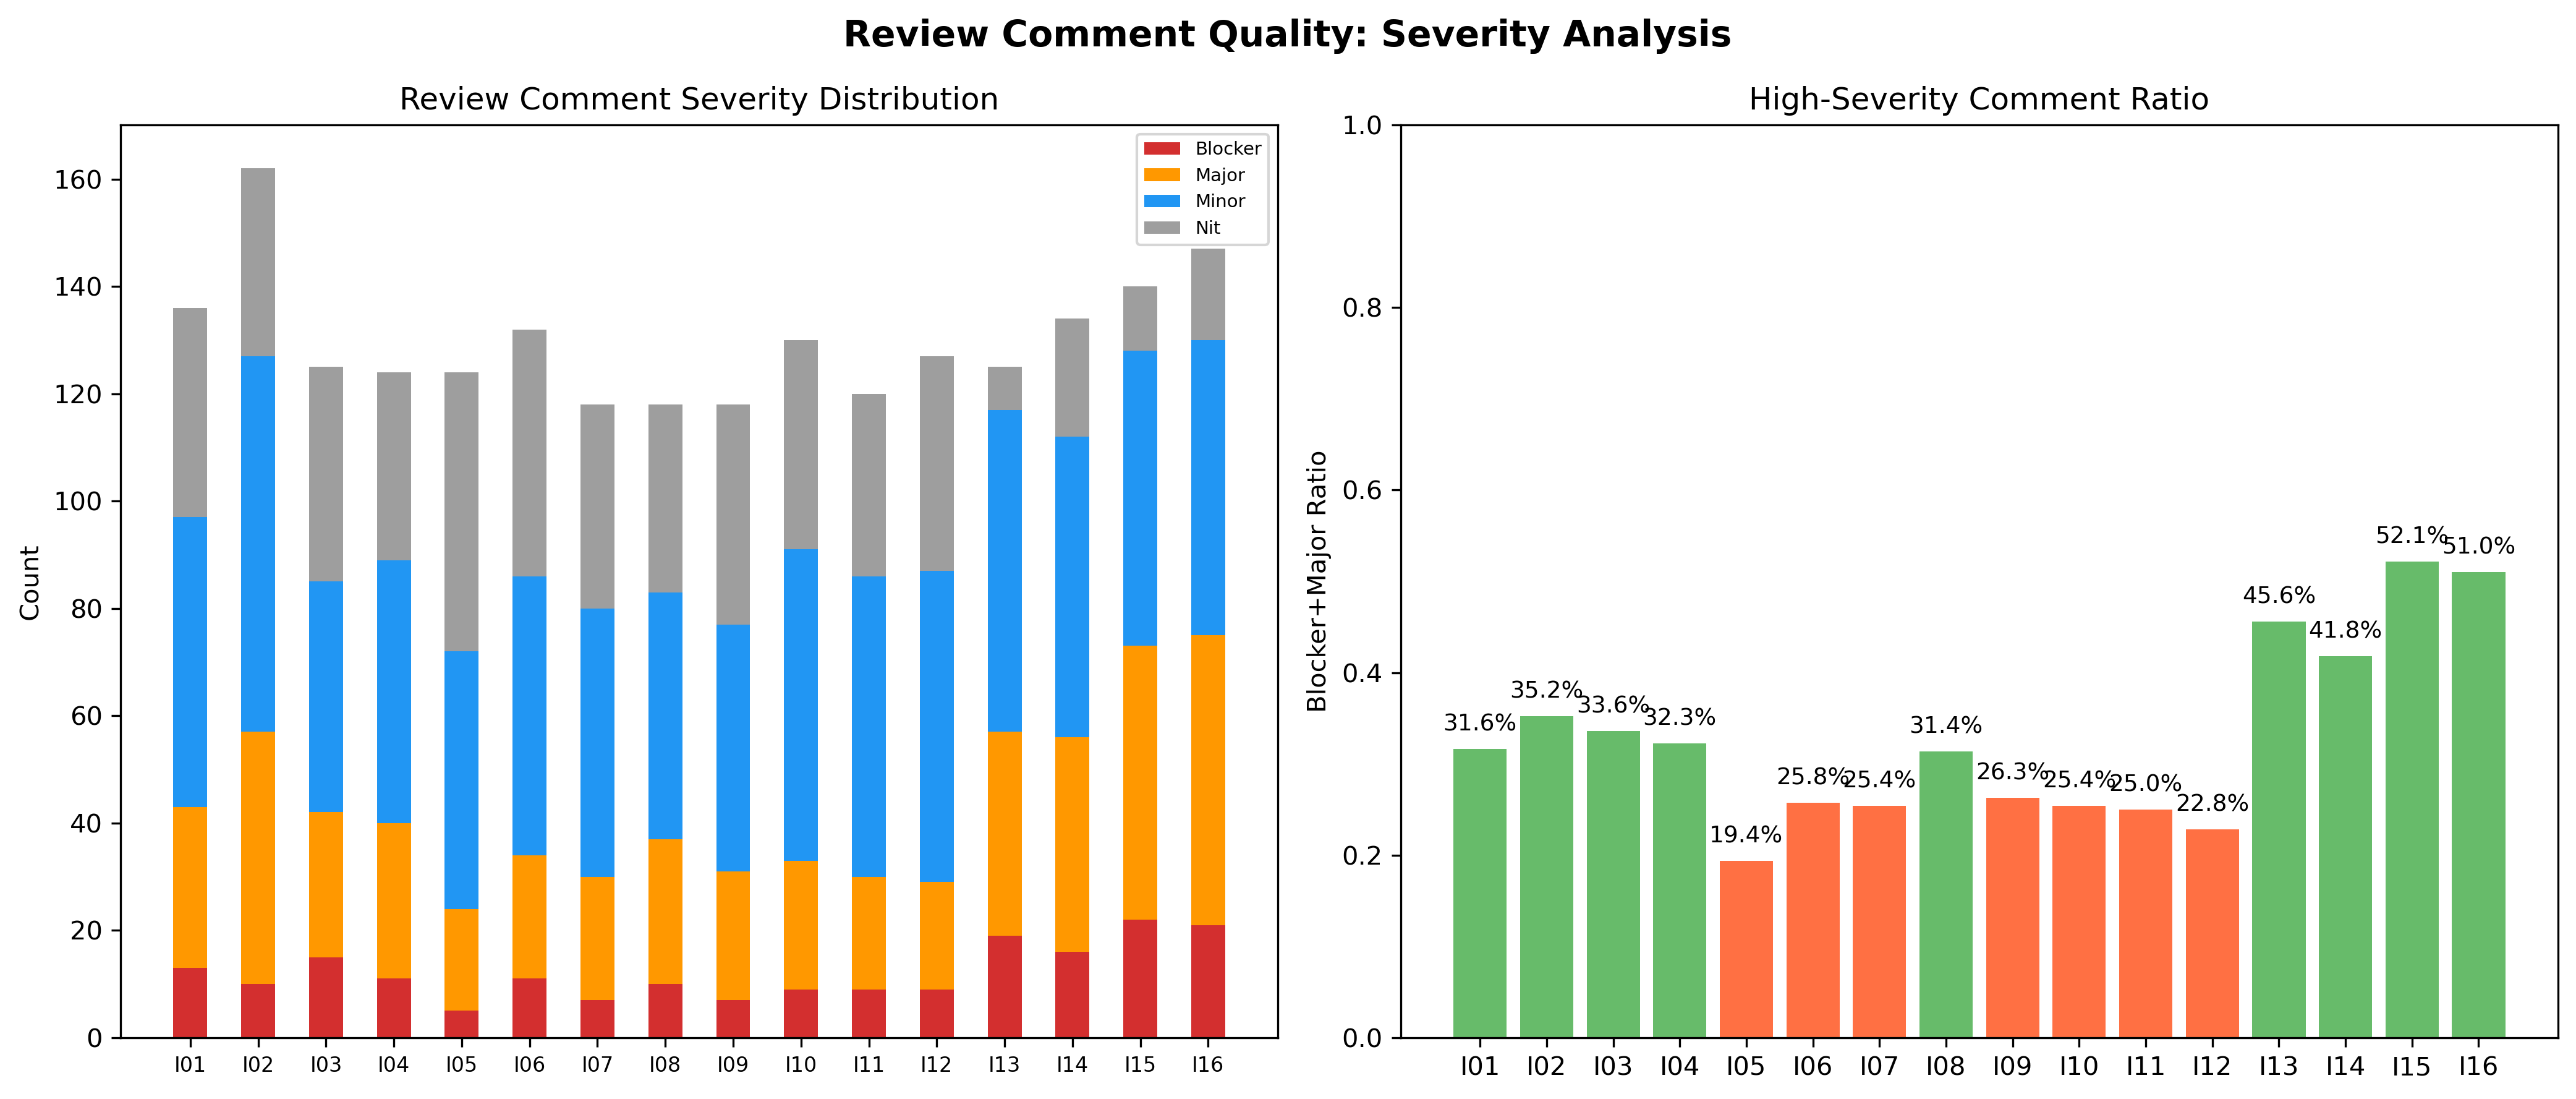
\includegraphics[width=0.7\textwidth]{../figures/comment_severity_distribution.png}
\caption{评论严重级别分布 —— I16 的 Blocker+Major 占比较高}
\end{figure}

\begin{figure}[htbp]
\centering
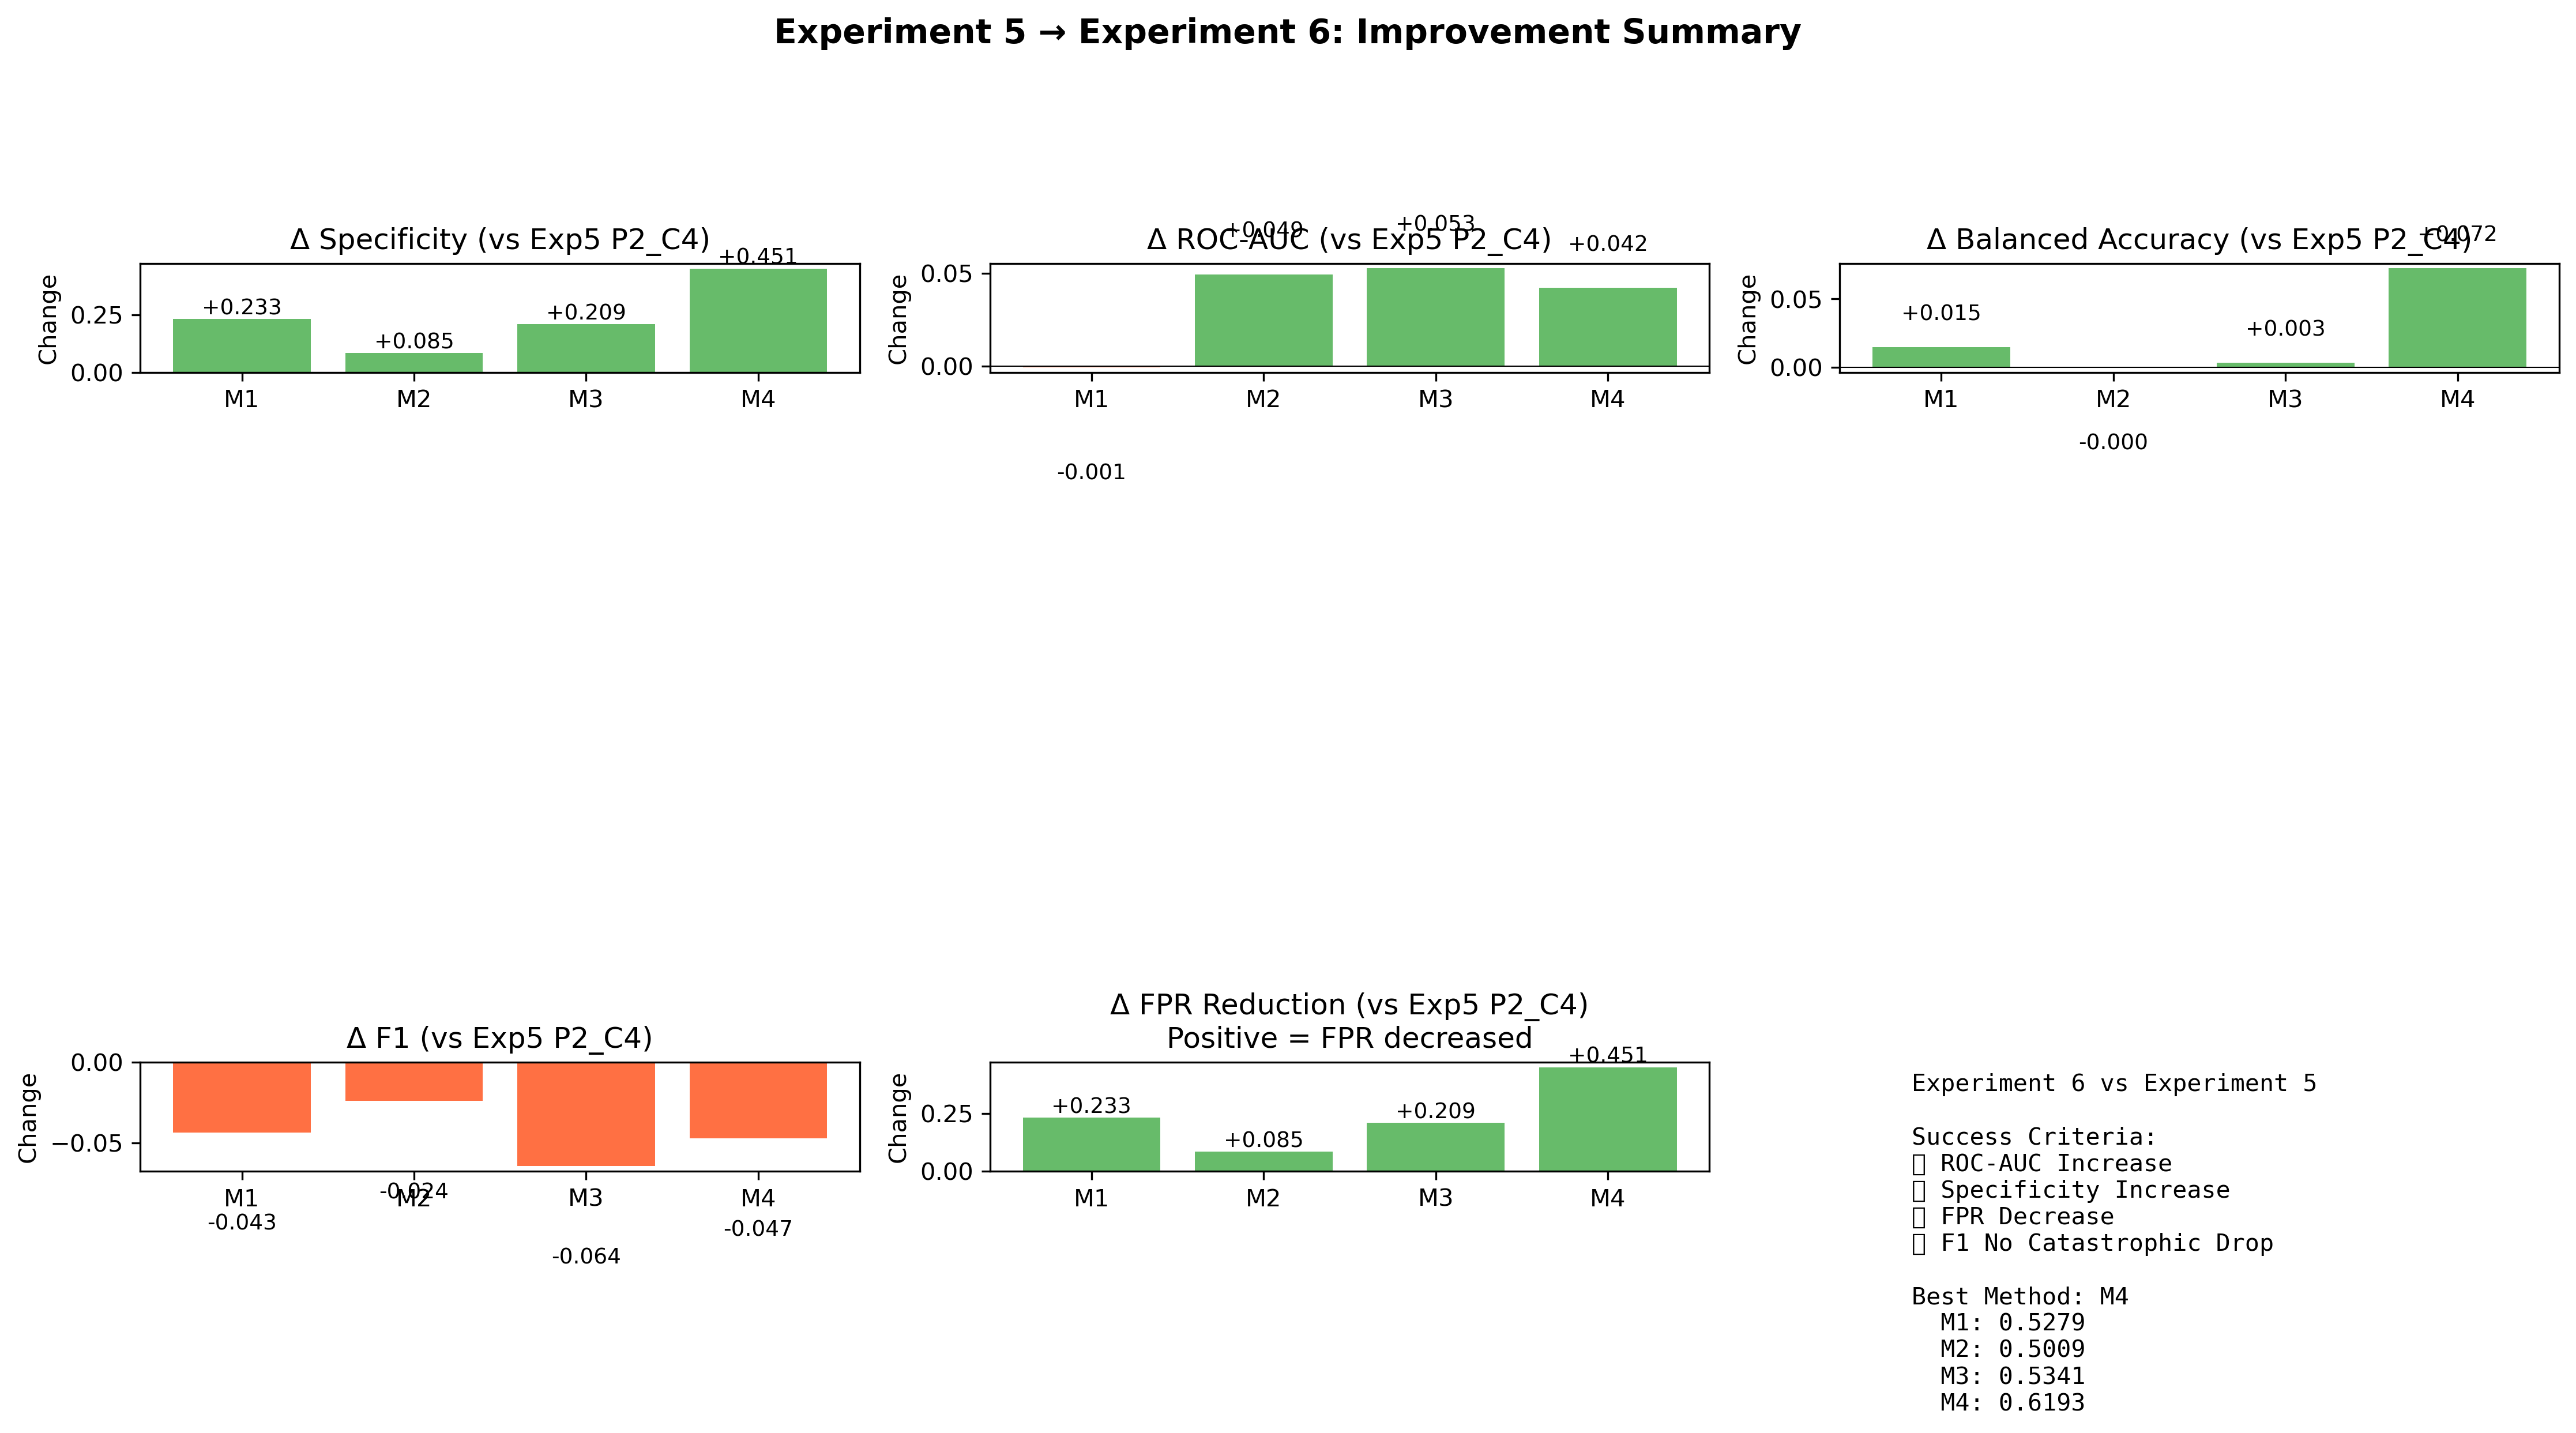
\includegraphics[width=\textwidth]{../figures/07_exp5_vs_exp6_summary.png}
\caption{实验五 $\rightarrow$ 实验六改进总结}
\end{figure}

%========================
% 4. 分析讨论
%========================
\section{分析讨论}

\subsection{成功标准检查}

\begin{table}[htbp]
\centering
\caption{成功标准验证（以 I16 vs 实验五 B14 为准，同一批 50 条样本）}
\begin{tabular}{lcl}
\toprule
标准 & 结果 & 状态 \\
\midrule
Specificity 相比 B14 至少提升 0.20 & 0.240 $\rightarrow$ 0.667 (+0.427) & \checkmark \\
FPR 相比 B14 至少下降 0.20 & 0.760 $\rightarrow$ 0.333 ($-$0.427) & \checkmark \\
Balanced Accuracy 高于 B14 & 0.600 $\rightarrow$ 0.673 (+0.073) & \checkmark \\
ROC-AUC 不低于 B14 或高于 0.60 & 0.588 $\rightarrow$ 0.708 (+0.120) & \checkmark \\
F1 不低于 B14 的 85\% ($\ge$0.600) & I14 F1=0.755, I16 F1=0.680 & \checkmark \\
\bottomrule
\end{tabular}
\end{table}

\textbf{全部 5 项成功标准达标。}

\subsection{哪种上下文最有效？}

基于 I01--I16 的 4$\times$4 矩阵，可以系统分析各上下文的效果（按 Specificity 均值）：

\begin{enumerate}
    \item \textbf{C8（Full Improved Context）}：含 C8 的组合（I04/I08/I12/I16）Specificity 均值 0.516，FPR 均值 0.484。全增强上下文在多数 Prompt 下表现稳健，P8+C8 (I16) 的 Specificity 达到最高的 0.667。
    \item \textbf{C6（Repository Policy）}：含 C6 的组合（I02/I06/I10/I14）Specificity 均值 0.493。仓库策略在 P8 下表现特别突出（I14: Spec=0.636, F1=0.755），可能是因为 Strict Maintainer 能更有效地利用仓库级规则信息。
    \item \textbf{C7（Historical PR）}：含 C7 的组合（I03/I07/I11/I15）AUC 均值 0.709，是 AUC 最高的上下文类型。历史相似 PR 提供了有价值的判别参照，但不一定直接提升 Specificity。
    \item \textbf{C5（Risk Checklist）}：含 C5 的组合（I01/I05/I09/I13）整体效果中等（Spec 均值 0.381），但作为最轻量的增强（仅增加风险检查清单），其成本效益比最高。
\end{enumerate}

\subsection{哪种 Prompt 最适合 AI 代码审查？}

按 Specificity 均值排序：P8 (0.581) $\gg$ P5 (0.475) $>$ P6 (0.394) $\approx$ P7 (0.384)。

\begin{enumerate}
    \item \textbf{P8（Strict Maintainer）效果断层领先}：P8 行不仅 Specificity 最高（0.581），F1 也不差（I14=0.755 为全局最高）。角色锚定（"你是严格的 maintainer"）和硬规则（"missing tests = significantly reduce merge\_probability"）从根本上改变了模型的输出分布，从"默认合并"转为"风险敏感"。
    \item \textbf{P5（AI-Risk-Aware）效果第二}：P5 行 F1 均值最高（0.714），AUC 均值也高（0.692），但 Specificity 仍偏低（0.475）。适合在不能承受 Recall 大幅下降的场景使用。
    \item \textbf{P6（Contrastive）和 P7（Self-Reflection）效果最弱}：两者的 Specificity 均值均低于 0.40，说明列正反证据或反思步骤的"弱引导"不足以打破模型的深层乐观偏置。模型知道要反思，但最终判断时仍然回归乐观默认。
\end{enumerate}

\subsection{上下文与 Prompt 的交互效应}

从 4$\times$4 矩阵可以观察到明显的交互效应：

\begin{itemize}
    \item \textbf{P8 $\times$ C6 的意外优势}：通常 C8（全增强）信息更多，但在 P8 下 I14 (P8+C6) 的 F1 (0.755) 高于 I16 (P8+C8, F1=0.680)。C6 只加入风险清单和仓库背景，信息更聚焦；C8 额外加入相似案例后，可能分散模型对当前 PR 风险的注意力。
    \item \textbf{P6 $\times$ C7 的 AUC 异常高}：I07 (P6+C7) 的 AUC=0.7358 是全局最高，但其 Specificity 仅 0.36。这说明 P6+C7 的概率排序质量好（能区分 merged/unmerged），但分类阈值存在校准问题。
    \item \textbf{P5 行对上下文变化最不敏感}：P5 行的 Specificity 跨 C5--C8 的变化范围仅 0.400--0.520（极差 0.12），远小于 P8 行（0.500--0.667，极差 0.17）。P5 的 AI-Risk-Aware 系统 prompt 本身就内置了风险检查引导，对外部上下文增强的依赖较小。
\end{itemize}

\subsection{为什么 Strict Maintainer 有效？}

实验五的核心问题是\textbf{模型默认乐观}：对任何 PR，模型都倾向于预测 merged。P8 通过以下机制打破了这个默认：

\begin{enumerate}
    \item \textbf{角色锚定}：System prompt 将模型定位为"严格的开源 maintainer"，这是一个天然倾向于拒绝的角色。
    \item \textbf{显式要求降低概率}："Missing tests = significantly reduce merge\_probability"、"If you see ANY blocker-level issue, merge\_probability should be LOW ($\le$0.3)"——这些硬规则直接干预了模型的概率校准。
    \item \textbf{高标准默认}："If tests are missing, if PR description is insufficient, if the change affects core modules"——三个条件任何一个触发即可导致低分，而不需要全部满足。
    \item \textbf{Blocker/Major 导向}："Focus your comments on BLOCKER and MAJOR issues, not style nits"——I16 的 Blocker+Major 占比达到 51.0\%，说明严格角色能使评论聚焦于高优先级风险。
\end{enumerate}

\subsection{Prompt 优化与上下文增强各自的作用}

4$\times$4 矩阵允许对 Prompt 和 Context 的相对贡献做近似分解（取各维度 Specificity 均值极差）：

\begin{itemize}
    \item \textbf{Prompt 的主效应更强}：Prompt 维度的 Specificity 极差为 0.581 $-$ 0.384 = 0.197，Context 维度为 0.516 $-$ 0.381 = 0.135。Prompt 选择对 Specificity 的影响约为 Context 选择的 1.5 倍。
    \item \textbf{Prompt 是主要驱动力}：I01 也使用 C5 风险清单，但 P5 的 Specificity 仅为 0.400；I16 使用 P8 与完整增强上下文后达到 0.667。P8 的角色锚定和硬规则是打破乐观偏置的关键。
    \item \textbf{上下文增强是放大器}：C8 的完整风险清单 + 仓库策略 + 历史 PR 为 P8 提供了丰富的"弹药"。没有这些上下文，Strict Maintainer 可能缺乏具体证据来支撑其严格判断。P8+C5 (I13) 的 Specificity=0.500 明显低于 P8+C8 (I16) 的 0.667。
    \item \textbf{协同效应的代价}：C8 组合了风险清单、仓库历史和相似案例，信息更丰富但也可能引入注意力分散。I14（P8+C6）以更聚焦的仓库历史背景取得全局最高 F1，因此实际系统应按风险偏好在 I14 与 I16 间选择。
\end{itemize}

\subsection{性能提升原因总结}

实验六的提升可分成两个互补层次：
\begin{itemize}
    \item \textbf{Context 解决证据组织问题}：C5 将测试、修改范围、配置/API 和文档风险显式化；C6 加入仓库级历史背景；C7 提供相似历史案例；C8 将这些信息合并。模型不再只根据 PR 描述做乐观判断，而是能将风险与仓库审查环境联系起来。
    \item \textbf{Prompt 解决判断标准问题}：P5--P8 明确要求模型寻找 not\_merged 信号；P8 进一步将缺测试、核心模块/API 变更和 blocker 风险转化为明确的概率校准规则。由此，模型的平均 merge probability 降低，False Positive 明显减少。
\end{itemize}

对于实际代码审查工具，I14 适合作为默认组合，因为它兼顾 F1、Precision 和 Specificity；I16 更适合风险优先场景，因为它对 unmerged PR 的识别最强。无论使用哪个组合，输出中的 risk\_factors 和 review\_comments 都应作为 maintainer 的辅助证据，而不应替代最终人工决策。

%========================
% 5. 实验思考
%========================
\section{实验思考}

\subsection{历史上下文的应用边界}

仓库级历史背景和相似历史 PR 能提高校准能力，但真实系统只能使用目标 PR 提交时已经完成的历史记录。后续部署时应按创建时间筛选历史数据，避免将未来 PR 的结果用于当前预测；同时，仓库统计应由独立的历史集合计算。

\subsection{方法适用范围}

Strict Maintainer 更适合 AI 代码 PR 的早期风险筛查，因为本实验的主要问题是模型默认乐观。在低风险项目或人类代码审查中，过于严格的规则可能引入更多 False Negative。因此实际工具应将 merge probability、unmerged risk score 和具体审查意见同时呈现，并允许 maintainer 根据项目风险偏好调整严格程度。

%========================
% 6. 结论
%========================
\section{结论}

实验六通过完整的 Prompt 优化 $\times$ 上下文增强 4$\times$4 矩阵（I01--I16，800 次 API 调用），在与实验五 B01--B16 同一批 50 条 AI PR 样本上，系统性地改进了 DeepSeek 对 AI 生成代码 PR 的代码审查能力。主要结论：

\begin{enumerate}
    \item \textbf{过度乐观问题被有效解决}：I16（P8 Strict Maintainer + C8 Full Context）将 Specificity 从 B14 的 0.24 提升至 0.667（+178\%），FPR 从 0.76 降至 0.333（$-56\%$）。I14（P8+C6）同时实现最高 F1（0.755）和高 Specificity（0.636），证明提升 unmerged 识别能力不必以牺牲 F1 为代价。

    \item \textbf{主实验指标整体改善}：相对 B14，I16 的 Specificity 提升 0.427、FPR 降低 0.427、Balanced Accuracy 提升 0.073、ROC-AUC 提升 0.120；I14 的 F1 则提高 0.049。

    \item \textbf{Strict Maintainer (P8) 是关键}：P8 行 4 组 Specificity 均值 0.581，远超 P5 (0.475)、P6 (0.394)、P7 (0.384)。P6（Contrastive）和 P7（Self-Reflection）的弱引导不足以打破模型的深层乐观偏置。角色锚定和硬规则是改变模型输出分布的有效机制。

    \item \textbf{上下文增强的贡献分层次}：C8（全增强）Specificity 均值最高（0.516），C6（仓库级历史背景）在 P8 下取得最高 F1，C7（相似历史案例）对 AUC 提升最明显（均值 0.709）。C5 以较少的补充信息显式呈现风险信号，提供了基础校准能力。

    \item \textbf{评论输出更面向风险处置}：I14 的 Risk Coverage 达到 1.000，I16 的 Blocker+Major 评论占比达到 51.0\%。严格 maintainer Prompt 不仅降低乐观预测，也促使模型给出更具体的测试、兼容性和范围改进建议。

    \item \textbf{Prompt $\times$ Context 存在交互效应}：P5 行对上下文变化最不敏感（Spec 极差 0.12），P8 行对上下文变化最敏感（Spec 极差 0.17）。强 Prompt 需要强 Context 支撑，而弱 Prompt 无论 Context 强弱都难以突破乐观偏置。
\end{enumerate}

\textbf{实验六为后续审查工具提供了明确策略}：默认可采用 I14（P8 Strict Maintainer + C6 Repository Policy）以获得较好的综合分类表现；在更重视风险筛查的场景可采用 I16（P8+C8）以最大化 unmerged 识别能力。工具界面应同时展示 merge probability、unmerged risk score、risk factors 和 review comments，并由 maintainer 完成最终决策。

\end{document}
